%%%%%%%%%%%%%%%%%%%%%%%%%%%%%%%%%%%%%%%%%
% Masters/Doctoral Thesis 
% LaTeX Template
% Version 2.5 (27/8/17)
%
% This template was downloaded from:
% http://www.LaTeXTemplates.com
%
% Version 2.x major modifications by:
% Vel (vel@latextemplates.com)
%
% This template is based on a template by:
% Steve Gunn (http://users.ecs.soton.ac.uk/srg/softwaretools/document/templates/)
% Sunil Patel (http://www.sunilpatel.co.uk/thesis-template/)
%
% Template license:
% CC BY-NC-SA 3.0 (http://creativecommons.org/licenses/by-nc-sa/3.0/)
%
%%%%%%%%%%%%%%%%%%%%%%%%%%%%%%%%%%%%%%%%%

%----------------------------------------------------------------------------------------
%	PACKAGES AND OTHER DOCUMENT CONFIGURATIONS
%----------------------------------------------------------------------------------------

\documentclass[
11pt, % The default document font size, options: 10pt, 11pt, 12pt
%oneside, % Two side (alternating margins) for binding by default, uncomment to switch to one side
english, % ngerman for German
singlespacing, % Single line spacing, alternatives: onehalfspacing or doublespacing
%draft, % Uncomment to enable draft mode (no pictures, no links, overfull hboxes indicated)
%nolistspacing, % If the document is onehalfspacing or doublespacing, uncomment this to set spacing in lists to single
%liststotoc, % Uncomment to add the list of figures/tables/etc to the table of contents
%toctotoc, % Uncomment to add the main table of contents to the table of contents
%parskip, % Uncomment to add space between paragraphs
%nohyperref, % Uncomment to not load the hyperref package
headsepline, % Uncomment to get a line under the header
%chapterinoneline, % Uncomment to place the chapter title next to the number on one line
%consistentlayout, % Uncomment to change the layout of the declaration, abstract and acknowledgements pages to match the default layout
]{MastersDoctoralThesis} % The class file specifying the document structure

\usepackage[utf8]{inputenc} % Required for inputting international characters
\usepackage[T1]{fontenc} % Output font encoding for international characters

\usepackage{mathpazo} % Use the Palatino font by default

\usepackage[backend=bibtex,style=numeric,natbib=true]{biblatex} % Use the bibtex backend with the authoryear citation style (which resembles APA)

\addbibresource{example.bib} % The filename of the bibliography

\usepackage[autostyle=true]{csquotes} % Required to generate language-dependent quotes in the bibliography

%----------------------------------------------------------------------------------------
%	MARGIN SETTINGS
%----------------------------------------------------------------------------------------

\geometry{
	paper=a4paper, % Change to letterpaper for US letter
	inner=2.5cm, % Inner margin
	outer=3.8cm, % Outer margin
	bindingoffset=.5cm, % Binding offset
	top=1.5cm, % Top margin
	bottom=1.5cm, % Bottom margin
	%showframe, % Uncomment to show how the type block is set on the page
}

%----------------------------------------------------------------------------------------
%	THESIS INFORMATION
%----------------------------------------------------------------------------------------

\thesistitle{A Deep Learning Library for FPGAs using OpenCL} % Your thesis title, this is used in the title and abstract, print it elsewhere with \ttitle
\supervisor{Dr. Torsten \textsc{Hoefler}} % Your supervisor's name, this is used in the title page, print it elsewhere with \supname
\examiner{} % Your examiner's name, this is not currently used anywhere in the template, print it elsewhere with \examname
\degree{Masters of Science in Computer Science} % Your degree name, this is used in the title page and abstract, print it elsewhere with \degreename
\author{Houssam \textsc{Naous}} % Your name, this is used in the title page and abstract, print it elsewhere with \authorname
\addresses{} % Your address, this is not currently used anywhere in the template, print it elsewhere with \addressname

\subject{Computer Science} % Your subject area, this is not currently used anywhere in the template, print it elsewhere with \subjectname
\keywords{} % Keywords for your thesis, this is not currently used anywhere in the template, print it elsewhere with \keywordnames
\university{\href{http://www.ethz.ch}{ETH Zürich}} % Your university's name and URL, this is used in the title page and abstract, print it elsewhere with \univname
\department{\href{https://www.inf.ethz.ch}{Computer Science}} % Your department's name and URL, this is used in the title page and abstract, print it elsewhere with \deptname
\group{\href{https://spcl.inf.ethz.ch}{Scalable and Parallel Computing Lab}} % Your research group's name and URL, this is used in the title page, print it elsewhere with \groupname
\faculty{\href{https://www.inf.ethz.ch}{Computer Science}} % Your faculty's name and URL, this is used in the title page and abstract, print it elsewhere with \facname

\AtBeginDocument{
\hypersetup{pdftitle=\ttitle} % Set the PDF's title to your title
\hypersetup{pdfauthor=\authorname} % Set the PDF's author to your name
\hypersetup{pdfkeywords=\keywordnames} % Set the PDF's keywords to your keywords
}

\begin{document}

\frontmatter % Use roman page numbering style (i, ii, iii, iv...) for the pre-content pages

\pagestyle{plain} % Default to the plain heading style until the thesis style is called for the body content

%----------------------------------------------------------------------------------------
%	TITLE PAGE
%----------------------------------------------------------------------------------------

\begin{titlepage}
\begin{center}

\vspace*{.06\textheight}
{\scshape\LARGE \univname\par}\vspace{1.5cm} % University name
\textsc{\Large Master's Thesis}\\[0.5cm] % Thesis type

\HRule \\[0.4cm] % Horizontal line
{\huge \bfseries \ttitle\par}\vspace{0.4cm} % Thesis title
\HRule \\[1.5cm] % Horizontal line
 
\begin{minipage}[t]{0.4\textwidth}
\begin{flushleft} \large
\emph{Author:}\\
\href{http://www.johnsmith.com}{\authorname} % Author name - remove the \href bracket to remove the link
\end{flushleft}
\end{minipage}
\begin{minipage}[t]{0.4\textwidth}
\begin{flushright} \large
\emph{Supervisor:} \\
\href{http://www.jamessmith.com}{\supname} % Supervisor name - remove the \href bracket to remove the link  
\end{flushright}
\end{minipage}\\[3cm]
 
\vfill

\large \textit{A thesis submitted in fulfillment of the requirements\\ for the degree of \degreename}\\[0.3cm] % University requirement text
\textit{in the}\\[0.4cm]
\groupname\\\deptname\\[2cm] % Research group name and department name
 
\vfill

{\large \today}\\[4cm] % Date
%\includegraphics{Logo} % University/department logo - uncomment to place it
 
\vfill
\end{center}
\end{titlepage}

%----------------------------------------------------------------------------------------
%	DECLARATION PAGE
%----------------------------------------------------------------------------------------

\begin{declaration}
\addchaptertocentry{\authorshipname} % Add the declaration to the table of contents
\noindent I, \authorname, declare that this thesis titled, \enquote{\ttitle} and the work presented in it are my own. I confirm that:

\begin{itemize} 
\item This work was done wholly or mainly while in candidature for a research degree at this University.
\item Where any part of this thesis has previously been submitted for a degree or any other qualification at this University or any other institution, this has been clearly stated.
\item Where I have consulted the published work of others, this is always clearly attributed.
\item Where I have quoted from the work of others, the source is always given. With the exception of such quotations, this thesis is entirely my own work.
\item I have acknowledged all main sources of help.
\item Where the thesis is based on work done by myself jointly with others, I have made clear exactly what was done by others and what I have contributed myself.\\
\end{itemize}
 
\noindent Signed:\\
\rule[0.5em]{25em}{0.5pt} % This prints a line for the signature
 
\noindent Date:\\
\rule[0.5em]{25em}{0.5pt} % This prints a line to write the date
\end{declaration}

\cleardoublepage

%----------------------------------------------------------------------------------------
%	QUOTATION PAGE
%----------------------------------------------------------------------------------------

\vspace*{0.2\textheight}

\noindent\enquote{\itshape Thanks to my solid academic training, today I can write hundreds of words on virtually any topic without possessing a shred of information, which is how I got a good job in journalism.}\bigbreak

\hfill Dave Barry

%----------------------------------------------------------------------------------------
%	ABSTRACT PAGE
%----------------------------------------------------------------------------------------

\begin{abstract}
\addchaptertocentry{\abstractname} % Add the abstract to the table of contents
The Thesis Abstract is written here (and usually kept to just this page). The page is kept centered vertically so can expand into the blank space above the title too\ldots
\end{abstract}

%----------------------------------------------------------------------------------------
%	ACKNOWLEDGEMENTS
%----------------------------------------------------------------------------------------

\begin{acknowledgements}
\addchaptertocentry{\acknowledgementname} % Add the acknowledgements to the table of contents
The acknowledgments and the people to thank go here, don't forget to include your project advisor\ldots
\end{acknowledgements}

%----------------------------------------------------------------------------------------
%	LIST OF CONTENTS/FIGURES/TABLES PAGES
%----------------------------------------------------------------------------------------

\tableofcontents % Prints the main table of contents

%\listoffigures % Prints the list of figures

%\listoftables % Prints the list of tables


%----------------------------------------------------------------------------------------
%	THESIS CONTENT - CHAPTERS
%----------------------------------------------------------------------------------------

\mainmatter % Begin numeric (1,2,3...) page numbering

\pagestyle{thesis} % Return the page headers back to the "thesis" style

% Include the chapters of the thesis as separate files from the Chapters folder
% Uncomment the lines as you write the chapters

% Chapter 1

\chapter{Chapter Title Here} % Main chapter title

\label{Chapter1} % For referencing the chapter elsewhere, use \ref{Chapter1} 

%----------------------------------------------------------------------------------------

% Define some commands to keep the formatting separated from the content 
\newcommand{\keyword}[1]{\textbf{#1}}
\newcommand{\tabhead}[1]{\textbf{#1}}
\newcommand{\code}[1]{\texttt{#1}}
\newcommand{\file}[1]{\texttt{\bfseries#1}}
\newcommand{\option}[1]{\texttt{\itshape#1}}

%----------------------------------------------------------------------------------------

\section{Welcome and Thank You}
Welcome to this \LaTeX{} Thesis Template, a beautiful and easy to use template for writing a thesis using the \LaTeX{} typesetting system.

If you are writing a thesis (or will be in the future) and its subject is technical or mathematical (though it doesn't have to be), then creating it in \LaTeX{} is highly recommended as a way to make sure you can just get down to the essential writing without having to worry over formatting or wasting time arguing with your word processor.

\LaTeX{} is easily able to professionally typeset documents that run to hundreds or thousands of pages long. With simple mark-up commands, it automatically sets out the table of contents, margins, page headers and footers and keeps the formatting consistent and beautiful. One of its main strengths is the way it can easily typeset mathematics, even \emph{heavy} mathematics. Even if those equations are the most horribly twisted and most difficult mathematical problems that can only be solved on a super-computer, you can at least count on \LaTeX{} to make them look stunning.

%----------------------------------------------------------------------------------------

\section{Learning \LaTeX{}}

\LaTeX{} is not a \textsc{wysiwyg} (What You See is What You Get) program, unlike word processors such as Microsoft Word or Apple's Pages. Instead, a document written for \LaTeX{} is actually a simple, plain text file that contains \emph{no formatting}. You tell \LaTeX{} how you want the formatting in the finished document by writing in simple commands amongst the text, for example, if I want to use \emph{italic text for emphasis}, I write the \verb|\emph{text}| command and put the text I want in italics in between the curly braces. This means that \LaTeX{} is a \enquote{mark-up} language, very much like HTML.

\subsection{A (not so short) Introduction to \LaTeX{}}

If you are new to \LaTeX{}, there is a very good eBook -- freely available online as a PDF file -- called, \enquote{The Not So Short Introduction to \LaTeX{}}. The book's title is typically shortened to just \emph{lshort}. You can download the latest version (as it is occasionally updated) from here:
\url{http://www.ctan.org/tex-archive/info/lshort/english/lshort.pdf}

It is also available in several other languages. Find yours from the list on this page: \url{http://www.ctan.org/tex-archive/info/lshort/}

It is recommended to take a little time out to learn how to use \LaTeX{} by creating several, small `test' documents, or having a close look at several templates on:\\ 
\url{http://www.LaTeXTemplates.com}\\ 
Making the effort now means you're not stuck learning the system when what you \emph{really} need to be doing is writing your thesis.

\subsection{A Short Math Guide for \LaTeX{}}

If you are writing a technical or mathematical thesis, then you may want to read the document by the AMS (American Mathematical Society) called, \enquote{A Short Math Guide for \LaTeX{}}. It can be found online here:
\url{http://www.ams.org/tex/amslatex.html}
under the \enquote{Additional Documentation} section towards the bottom of the page.

\subsection{Common \LaTeX{} Math Symbols}
There are a multitude of mathematical symbols available for \LaTeX{} and it would take a great effort to learn the commands for them all. The most common ones you are likely to use are shown on this page:
\url{http://www.sunilpatel.co.uk/latex-type/latex-math-symbols/}

You can use this page as a reference or crib sheet, the symbols are rendered as large, high quality images so you can quickly find the \LaTeX{} command for the symbol you need.

\subsection{\LaTeX{} on a Mac}
 
The \LaTeX{} distribution is available for many systems including Windows, Linux and Mac OS X. The package for OS X is called MacTeX and it contains all the applications you need -- bundled together and pre-customized -- for a fully working \LaTeX{} environment and work flow.
 
MacTeX includes a custom dedicated \LaTeX{} editor called TeXShop for writing your `\file{.tex}' files and BibDesk: a program to manage your references and create your bibliography section just as easily as managing songs and creating playlists in iTunes.

%----------------------------------------------------------------------------------------

\section{Getting Started with this Template}

If you are familiar with \LaTeX{}, then you should explore the directory structure of the template and then proceed to place your own information into the \emph{THESIS INFORMATION} block of the \file{main.tex} file. You can then modify the rest of this file to your unique specifications based on your degree/university. Section \ref{FillingFile} on page \pageref{FillingFile} will help you do this. Make sure you also read section \ref{ThesisConventions} about thesis conventions to get the most out of this template.

If you are new to \LaTeX{} it is recommended that you carry on reading through the rest of the information in this document.

Before you begin using this template you should ensure that its style complies with the thesis style guidelines imposed by your institution. In most cases this template style and layout will be suitable. If it is not, it may only require a small change to bring the template in line with your institution's recommendations. These modifications will need to be done on the \file{MastersDoctoralThesis.cls} file.

\subsection{About this Template}

This \LaTeX{} Thesis Template is originally based and created around a \LaTeX{} style file created by Steve R.\ Gunn from the University of Southampton (UK), department of Electronics and Computer Science. You can find his original thesis style file at his site, here:
\url{http://www.ecs.soton.ac.uk/~srg/softwaretools/document/templates/}

Steve's \file{ecsthesis.cls} was then taken by Sunil Patel who modified it by creating a skeleton framework and folder structure to place the thesis files in. The resulting template can be found on Sunil's site here:
\url{http://www.sunilpatel.co.uk/thesis-template}

Sunil's template was made available through \url{http://www.LaTeXTemplates.com} where it was modified many times based on user requests and questions. Version 2.0 and onwards of this template represents a major modification to Sunil's template and is, in fact, hardly recognisable. The work to make version 2.0 possible was carried out by \href{mailto:vel@latextemplates.com}{Vel} and Johannes Böttcher.

%----------------------------------------------------------------------------------------

\section{What this Template Includes}

\subsection{Folders}

This template comes as a single zip file that expands out to several files and folders. The folder names are mostly self-explanatory:

\keyword{Appendices} -- this is the folder where you put the appendices. Each appendix should go into its own separate \file{.tex} file. An example and template are included in the directory.

\keyword{Chapters} -- this is the folder where you put the thesis chapters. A thesis usually has about six chapters, though there is no hard rule on this. Each chapter should go in its own separate \file{.tex} file and they can be split as:
\begin{itemize}
\item Chapter 1: Introduction to the thesis topic
\item Chapter 2: Background information and theory
\item Chapter 3: (Laboratory) experimental setup
\item Chapter 4: Details of experiment 1
\item Chapter 5: Details of experiment 2
\item Chapter 6: Discussion of the experimental results
\item Chapter 7: Conclusion and future directions
\end{itemize}
This chapter layout is specialised for the experimental sciences, your discipline may be different.

\keyword{Figures} -- this folder contains all figures for the thesis. These are the final images that will go into the thesis document.

\subsection{Files}

Included are also several files, most of them are plain text and you can see their contents in a text editor. After initial compilation, you will see that more auxiliary files are created by \LaTeX{} or BibTeX and which you don't need to delete or worry about:

\keyword{example.bib} -- this is an important file that contains all the bibliographic information and references that you will be citing in the thesis for use with BibTeX. You can write it manually, but there are reference manager programs available that will create and manage it for you. Bibliographies in \LaTeX{} are a large subject and you may need to read about BibTeX before starting with this. Many modern reference managers will allow you to export your references in BibTeX format which greatly eases the amount of work you have to do.

\keyword{MastersDoctoralThesis.cls} -- this is an important file. It is the class file that tells \LaTeX{} how to format the thesis. 

\keyword{main.pdf} -- this is your beautifully typeset thesis (in the PDF file format) created by \LaTeX{}. It is supplied in the PDF with the template and after you compile the template you should get an identical version.

\keyword{main.tex} -- this is an important file. This is the file that you tell \LaTeX{} to compile to produce your thesis as a PDF file. It contains the framework and constructs that tell \LaTeX{} how to layout the thesis. It is heavily commented so you can read exactly what each line of code does and why it is there. After you put your own information into the \emph{THESIS INFORMATION} block -- you have now started your thesis!

Files that are \emph{not} included, but are created by \LaTeX{} as auxiliary files include:

\keyword{main.aux} -- this is an auxiliary file generated by \LaTeX{}, if it is deleted \LaTeX{} simply regenerates it when you run the main \file{.tex} file.

\keyword{main.bbl} -- this is an auxiliary file generated by BibTeX, if it is deleted, BibTeX simply regenerates it when you run the \file{main.aux} file. Whereas the \file{.bib} file contains all the references you have, this \file{.bbl} file contains the references you have actually cited in the thesis and is used to build the bibliography section of the thesis.

\keyword{main.blg} -- this is an auxiliary file generated by BibTeX, if it is deleted BibTeX simply regenerates it when you run the main \file{.aux} file.

\keyword{main.lof} -- this is an auxiliary file generated by \LaTeX{}, if it is deleted \LaTeX{} simply regenerates it when you run the main \file{.tex} file. It tells \LaTeX{} how to build the \emph{List of Figures} section.

\keyword{main.log} -- this is an auxiliary file generated by \LaTeX{}, if it is deleted \LaTeX{} simply regenerates it when you run the main \file{.tex} file. It contains messages from \LaTeX{}, if you receive errors and warnings from \LaTeX{}, they will be in this \file{.log} file.

\keyword{main.lot} -- this is an auxiliary file generated by \LaTeX{}, if it is deleted \LaTeX{} simply regenerates it when you run the main \file{.tex} file. It tells \LaTeX{} how to build the \emph{List of Tables} section.

\keyword{main.out} -- this is an auxiliary file generated by \LaTeX{}, if it is deleted \LaTeX{} simply regenerates it when you run the main \file{.tex} file.

So from this long list, only the files with the \file{.bib}, \file{.cls} and \file{.tex} extensions are the most important ones. The other auxiliary files can be ignored or deleted as \LaTeX{} and BibTeX will regenerate them.

%----------------------------------------------------------------------------------------

\section{Filling in Your Information in the \file{main.tex} File}\label{FillingFile}

You will need to personalise the thesis template and make it your own by filling in your own information. This is done by editing the \file{main.tex} file in a text editor or your favourite LaTeX environment.

Open the file and scroll down to the third large block titled \emph{THESIS INFORMATION} where you can see the entries for \emph{University Name}, \emph{Department Name}, etc \ldots

Fill out the information about yourself, your group and institution. You can also insert web links, if you do, make sure you use the full URL, including the \code{http://} for this. If you don't want these to be linked, simply remove the \verb|\href{url}{name}| and only leave the name.

When you have done this, save the file and recompile \code{main.tex}. All the information you filled in should now be in the PDF, complete with web links. You can now begin your thesis proper!

%----------------------------------------------------------------------------------------

\section{The \code{main.tex} File Explained}

The \file{main.tex} file contains the structure of the thesis. There are plenty of written comments that explain what pages, sections and formatting the \LaTeX{} code is creating. Each major document element is divided into commented blocks with titles in all capitals to make it obvious what the following bit of code is doing. Initially there seems to be a lot of \LaTeX{} code, but this is all formatting, and it has all been taken care of so you don't have to do it.

Begin by checking that your information on the title page is correct. For the thesis declaration, your institution may insist on something different than the text given. If this is the case, just replace what you see with what is required in the \emph{DECLARATION PAGE} block.

Then comes a page which contains a funny quote. You can put your own, or quote your favourite scientist, author, person, and so on. Make sure to put the name of the person who you took the quote from.

Following this is the abstract page which summarises your work in a condensed way and can almost be used as a standalone document to describe what you have done. The text you write will cause the heading to move up so don't worry about running out of space.

Next come the acknowledgements. On this page, write about all the people who you wish to thank (not forgetting parents, partners and your advisor/supervisor).

The contents pages, list of figures and tables are all taken care of for you and do not need to be manually created or edited. The next set of pages are more likely to be optional and can be deleted since they are for a more technical thesis: insert a list of abbreviations you have used in the thesis, then a list of the physical constants and numbers you refer to and finally, a list of mathematical symbols used in any formulae. Making the effort to fill these tables means the reader has a one-stop place to refer to instead of searching the internet and references to try and find out what you meant by certain abbreviations or symbols.

The list of symbols is split into the Roman and Greek alphabets. Whereas the abbreviations and symbols ought to be listed in alphabetical order (and this is \emph{not} done automatically for you) the list of physical constants should be grouped into similar themes.

The next page contains a one line dedication. Who will you dedicate your thesis to?

Finally, there is the block where the chapters are included. Uncomment the lines (delete the \code{\%} character) as you write the chapters. Each chapter should be written in its own file and put into the \emph{Chapters} folder and named \file{Chapter1}, \file{Chapter2}, etc\ldots Similarly for the appendices, uncomment the lines as you need them. Each appendix should go into its own file and placed in the \emph{Appendices} folder.

After the preamble, chapters and appendices finally comes the bibliography. The bibliography style (called \option{authoryear}) is used for the bibliography and is a fully featured style that will even include links to where the referenced paper can be found online. Do not underestimate how grateful your reader will be to find that a reference to a paper is just a click away. Of course, this relies on you putting the URL information into the BibTeX file in the first place.

%----------------------------------------------------------------------------------------

\section{Thesis Features and Conventions}\label{ThesisConventions}

To get the best out of this template, there are a few conventions that you may want to follow.

One of the most important (and most difficult) things to keep track of in such a long document as a thesis is consistency. Using certain conventions and ways of doing things (such as using a Todo list) makes the job easier. Of course, all of these are optional and you can adopt your own method.

\subsection{Printing Format}

This thesis template is designed for double sided printing (i.e. content on the front and back of pages) as most theses are printed and bound this way. Switching to one sided printing is as simple as uncommenting the \option{oneside} option of the \code{documentclass} command at the top of the \file{main.tex} file. You may then wish to adjust the margins to suit specifications from your institution.

The headers for the pages contain the page number on the outer side (so it is easy to flick through to the page you want) and the chapter name on the inner side.

The text is set to 11 point by default with single line spacing, again, you can tune the text size and spacing should you want or need to using the options at the very start of \file{main.tex}. The spacing can be changed similarly by replacing the \option{singlespacing} with \option{onehalfspacing} or \option{doublespacing}.

\subsection{Using US Letter Paper}

The paper size used in the template is A4, which is the standard size in Europe. If you are using this thesis template elsewhere and particularly in the United States, then you may have to change the A4 paper size to the US Letter size. This can be done in the margins settings section in \file{main.tex}.

Due to the differences in the paper size, the resulting margins may be different to what you like or require (as it is common for institutions to dictate certain margin sizes). If this is the case, then the margin sizes can be tweaked by modifying the values in the same block as where you set the paper size. Now your document should be set up for US Letter paper size with suitable margins.

\subsection{References}

The \code{biblatex} package is used to format the bibliography and inserts references such as this one \parencite{Reference1}. The options used in the \file{main.tex} file mean that the in-text citations of references are formatted with the author(s) listed with the date of the publication. Multiple references are separated by semicolons (e.g. \parencite{Reference2, Reference1}) and references with more than three authors only show the first author with \emph{et al.} indicating there are more authors (e.g. \parencite{Reference3}). This is done automatically for you. To see how you use references, have a look at the \file{Chapter1.tex} source file. Many reference managers allow you to simply drag the reference into the document as you type.

Scientific references should come \emph{before} the punctuation mark if there is one (such as a comma or period). The same goes for footnotes\footnote{Such as this footnote, here down at the bottom of the page.}. You can change this but the most important thing is to keep the convention consistent throughout the thesis. Footnotes themselves should be full, descriptive sentences (beginning with a capital letter and ending with a full stop). The APA6 states: \enquote{Footnote numbers should be superscripted, [...], following any punctuation mark except a dash.} The Chicago manual of style states: \enquote{A note number should be placed at the end of a sentence or clause. The number follows any punctuation mark except the dash, which it precedes. It follows a closing parenthesis.}

The bibliography is typeset with references listed in alphabetical order by the first author's last name. This is similar to the APA referencing style. To see how \LaTeX{} typesets the bibliography, have a look at the very end of this document (or just click on the reference number links in in-text citations).

\subsubsection{A Note on bibtex}

The bibtex backend used in the template by default does not correctly handle unicode character encoding (i.e. "international" characters). You may see a warning about this in the compilation log and, if your references contain unicode characters, they may not show up correctly or at all. The solution to this is to use the biber backend instead of the outdated bibtex backend. This is done by finding this in \file{main.tex}: \option{backend=bibtex} and changing it to \option{backend=biber}. You will then need to delete all auxiliary BibTeX files and navigate to the template directory in your terminal (command prompt). Once there, simply type \code{biber main} and biber will compile your bibliography. You can then compile \file{main.tex} as normal and your bibliography will be updated. An alternative is to set up your LaTeX editor to compile with biber instead of bibtex, see \href{http://tex.stackexchange.com/questions/154751/biblatex-with-biber-configuring-my-editor-to-avoid-undefined-citations/}{here} for how to do this for various editors.

\subsection{Tables}

Tables are an important way of displaying your results, below is an example table which was generated with this code:

{\small
\begin{verbatim}
\begin{table}
\caption{The effects of treatments X and Y on the four groups studied.}
\label{tab:treatments}
\centering
\begin{tabular}{l l l}
\toprule
\tabhead{Groups} & \tabhead{Treatment X} & \tabhead{Treatment Y} \\
\midrule
1 & 0.2 & 0.8\\
2 & 0.17 & 0.7\\
3 & 0.24 & 0.75\\
4 & 0.68 & 0.3\\
\bottomrule\\
\end{tabular}
\end{table}
\end{verbatim}
}

\begin{table}
\caption{The effects of treatments X and Y on the four groups studied.}
\label{tab:treatments}
\centering
\begin{tabular}{l l l}
\toprule
\tabhead{Groups} & \tabhead{Treatment X} & \tabhead{Treatment Y} \\
\midrule
1 & 0.2 & 0.8\\
2 & 0.17 & 0.7\\
3 & 0.24 & 0.75\\
4 & 0.68 & 0.3\\
\bottomrule\\
\end{tabular}
\end{table}

You can reference tables with \verb|\ref{<label>}| where the label is defined within the table environment. See \file{Chapter1.tex} for an example of the label and citation (e.g. Table~\ref{tab:treatments}).

\subsection{Figures}

There will hopefully be many figures in your thesis (that should be placed in the \emph{Figures} folder). The way to insert figures into your thesis is to use a code template like this:
\begin{verbatim}
\begin{figure}
\centering

\includegraphics{Figures/Electron}
\decoRule
\caption[An Electron]{An electron (artist's impression).}
\label{fig:Electron}
\end{figure}
\end{verbatim}
Also look in the source file. Putting this code into the source file produces the picture of the electron that you can see in the figure below.

\begin{figure}[th]
\centering

\includegraphics{Figures/Electron}
\decoRule
\caption[An Electron]{An electron (artist's impression).}
\label{fig:Electron}
\end{figure}

Sometimes figures don't always appear where you write them in the source. The placement depends on how much space there is on the page for the figure. Sometimes there is not enough room to fit a figure directly where it should go (in relation to the text) and so \LaTeX{} puts it at the top of the next page. Positioning figures is the job of \LaTeX{} and so you should only worry about making them look good!

Figures usually should have captions just in case you need to refer to them (such as in Figure~\ref{fig:Electron}). The \verb|\caption| command contains two parts, the first part, inside the square brackets is the title that will appear in the \emph{List of Figures}, and so should be short. The second part in the curly brackets should contain the longer and more descriptive caption text.

The \verb|\decoRule| command is optional and simply puts an aesthetic horizontal line below the image. If you do this for one image, do it for all of them.

\LaTeX{} is capable of using images in pdf, jpg and png format.

\subsection{Typesetting mathematics}

If your thesis is going to contain heavy mathematical content, be sure that \LaTeX{} will make it look beautiful, even though it won't be able to solve the equations for you.

The \enquote{Not So Short Introduction to \LaTeX} (available on \href{http://www.ctan.org/tex-archive/info/lshort/english/lshort.pdf}{CTAN}) should tell you everything you need to know for most cases of typesetting mathematics. If you need more information, a much more thorough mathematical guide is available from the AMS called, \enquote{A Short Math Guide to \LaTeX} and can be downloaded from:
\url{ftp://ftp.ams.org/pub/tex/doc/amsmath/short-math-guide.pdf}

There are many different \LaTeX{} symbols to remember, luckily you can find the most common symbols in \href{http://ctan.org/pkg/comprehensive}{The Comprehensive \LaTeX~Symbol List}.

You can write an equation, which is automatically given an equation number by \LaTeX{} like this:
\begin{verbatim}
\begin{equation}
E = mc^{2}
\label{eqn:Einstein}
\end{equation}
\end{verbatim}

This will produce Einstein's famous energy-matter equivalence equation:
\begin{equation}
E = mc^{2}
\label{eqn:Einstein}
\end{equation}

All equations you write (which are not in the middle of paragraph text) are automatically given equation numbers by \LaTeX{}. If you don't want a particular equation numbered, use the unnumbered form:
\begin{verbatim}
\[ a^{2}=4 \]
\end{verbatim}

%----------------------------------------------------------------------------------------

\section{Sectioning and Subsectioning}

You should break your thesis up into nice, bite-sized sections and subsections. \LaTeX{} automatically builds a table of Contents by looking at all the \verb|\chapter{}|, \verb|\section{}|  and \verb|\subsection{}| commands you write in the source.

The Table of Contents should only list the sections to three (3) levels. A \verb|chapter{}| is level zero (0). A \verb|\section{}| is level one (1) and so a \verb|\subsection{}| is level two (2). In your thesis it is likely that you will even use a \verb|subsubsection{}|, which is level three (3). The depth to which the Table of Contents is formatted is set within \file{MastersDoctoralThesis.cls}. If you need this changed, you can do it in \file{main.tex}.

%----------------------------------------------------------------------------------------

\section{In Closing}

You have reached the end of this mini-guide. You can now rename or overwrite this pdf file and begin writing your own \file{Chapter1.tex} and the rest of your thesis. The easy work of setting up the structure and framework has been taken care of for you. It's now your job to fill it out!

Good luck and have lots of fun!

\begin{flushright}
Guide written by ---\\
Sunil Patel: \href{http://www.sunilpatel.co.uk}{www.sunilpatel.co.uk}\\
Vel: \href{http://www.LaTeXTemplates.com}{LaTeXTemplates.com}
\end{flushright}

% Chapter 2

\chapter{Deep Neural Networks and Parallelism} % Main chapter title

\label{Chapter2} % For referencing the chapter elsewhere, use \ref{Chapter2} 

%----------------------------------------------------------------------------------------
\section{Deep Learning Applications}

Deep learning and the progress made in the field have all fueled its integration into many applications of daily life \cite{ddl}. In the early days, the results of machine learning were dependent on the quality and informativeness of the features fed into the learning algorithm \cite{csaji2001approximation}. With the development of deep neural nets, the machine itself can abstract raw data and learn complex features that become much more informative than the hand-engineered ones. Modern architectures are able to process and incoming stream of images, video, or speech and learn to classify those raw data and solve complex problems in image segmentation and speech recognition \cite{lecun2015deep, resnet, densenet}. What is also important is that the value gained by those architectures increases as more data and more computational resources are presented to the network for training. Learning can be supervised, semi-supervised, and unsupervised \cite{lecun2015deep}. Supervised learning is a problem of finding the best mapping between a set of input data $\mathit{X}$ and a set of output labels or values $\mathit{Y}$. The algorithm proceeds in approximating the mapping function $\mathit{ f : X \rightarrow Y}$ by observing both the inputs and the labels and learning stops when an acceptable approximation of $\mathit{f}$ is found. Supervised learning can be split into two categories; classification when the output variable is a given label as in objects : \emph{"table"} , \emph{“chair”} , or \emph{“motorcycle”}, and regression when the output variable is a real-value such as \emph{"temperature"} or \emph{"dollar value"}. The goal of unsupervised learning on the other hand is to discover a data model or structure of the given data. There are no given labels or output variables and the goals is to learn something useful about the data. Unsupervised learning is split also into two categories; clustering by splitting the data into groups having similar attributes, and association where we want to discover rules that describe a large subset of the observed data ( ex. People who work at \emph{"X"} tend to buy product \emph{"Y"} ). Semi-supervised learning is situated somewhere in between supervised and unsupervised learning where only a subset of the data is labeled. Solving these problems requires both supervised techniques to label the unlabelled data and feed back in the labels for training, or the data can be used to uncover structure. Our work focuses more on supervised learning as the majority of deployed applications use supervised learning. We attempt to accelerate and develop an FPGA accelerator for training deep neural networks. 

%----------------------------------------------------------------------------------------
\section{Convolutional Neural Networks}

Convolutional Neural Networks have achieved many successes in multidimensional data than can be represented as arrays. A typical image can be represented as a three-channeled ( Red, Green, and Blue ) two-dimensional array of varying pixel intensities. A convolutional neural net is mainly composed of two stages that make sense of structured grid-like data to accomplish a learning task such as classification, regression, or even dimensionality reduction. An initial stage of convolution operators that pass a window filter over the image to extract an output feature map as in a discrete convolution operator. The convolution operation was inspired by a cat’s visual cortex and how neurons in the brain are triggered by certain shapes like lines in the seen image \cite{hubel1962receptive}. The intuition behind the convolution operation as a feature extraction method is that nearby pixels exhibit similarities and show high correlations. Also the image patches extracted in the convolution windows which represent concepts can appear anywhere elsewhere in the image. The convolution layers are usually followed by non-linear activations and then pooling operators. The role of pooling layers is to merge the similar nearby features into one to decrease the sensitivity of the network to the position of the extracted feature \cite{szegedy2015going}. The second stage of a CNN is a series of fully connected layers ultimately terminating at an output layer.

\subsection{Case Study : LeNet-5}
The Lenet \cite{lenet} is considered to be the first demonstration of a convolutional neural network and was proposed by LeCun et. al \cite{lenet} in 1998. Its architecture has shown record accuracy in classifying digits and was deployed commercially for identifying characters on personal and business checks. Le Cunn’s work was the first to demonstrate the benefit of brute-force numerical tricks in convolutions and that these tricks can be more useful than hand-engineering traditional feature engineering techniques. Also compared to traditional neural networks, the convolution layers are more robust as the extracted features are shift and translation invariant. This proved to be efficient since handwritten characters differ in slant and scale from one person’s handwriting to another’s and it was hard back then to perform feature preprocessing to documents such as normalization and centering handwritten characters.

\subsubsection{Architecture}

\begin{figure}[h!]
\centering
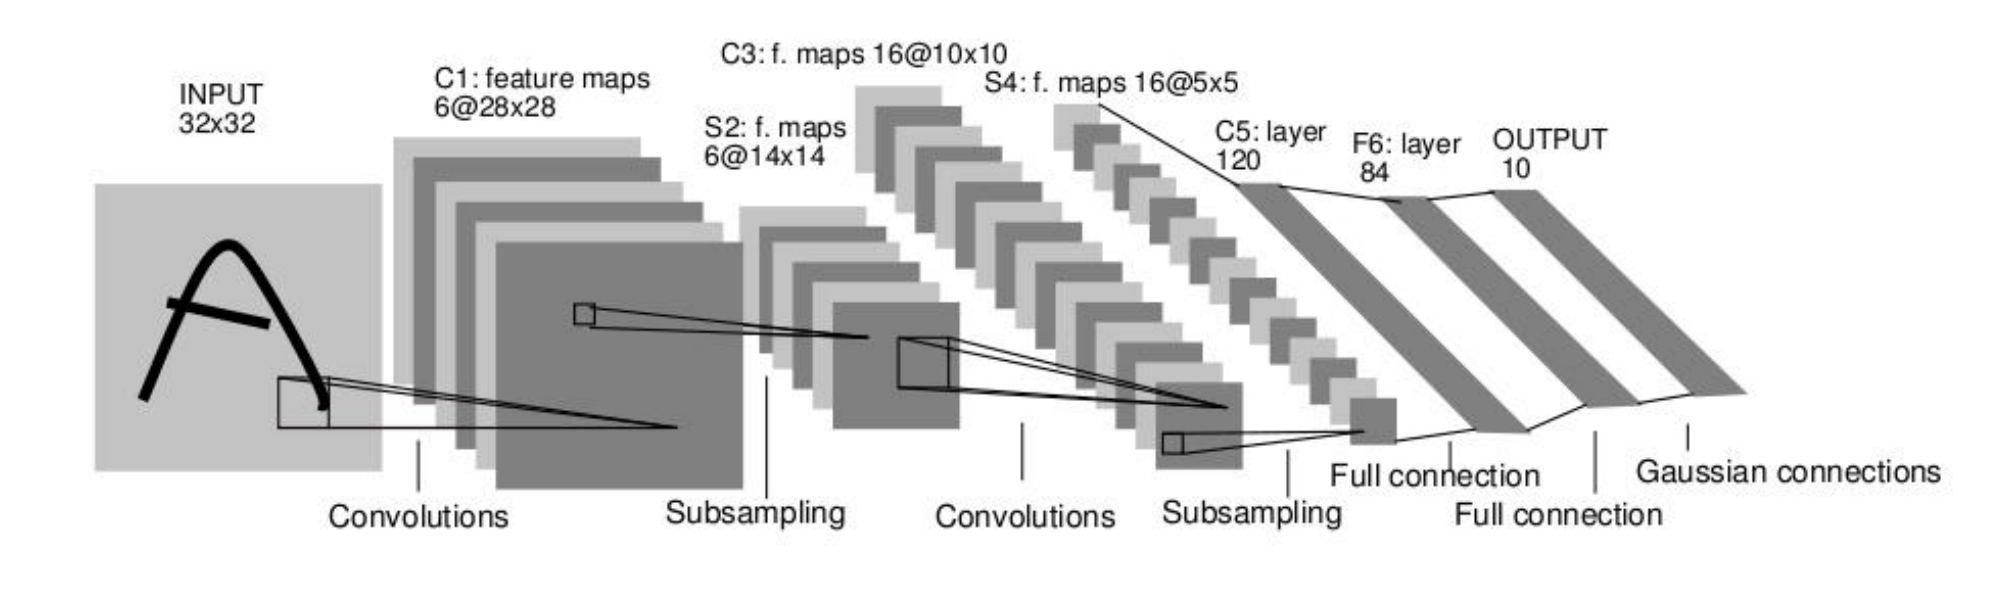
\includegraphics[width=1.0\textwidth]{Figures/lenet}
\decoRule
\caption[LeNet]{ LeNet-5 Architecture, a convolutional neural network used for character recognition. \cite{lenet}}
\label{fig:Lenet-5}
\end{figure}

The Lenet-5 is comprised of 7 layers ( excluding the input layer ), all of which contain trainable parameters. The input is a centered 32x32 image which represents the raw data that is fed into the network. It is followed by a convolutional layer and a subsampling layer. The first convolutional layer C1 produces an output of 6 distinct feature maps. Each feature map is obtained by sliding a 5x5 filter along the input image and computing a weighted sum of the pixels inside the window. This leads to shrinking the image by 4 pixels along both dimensions, and 6 features are obtained by passing 6 different weights for the filters. A bias is added to the weighted sum of pixels and it is squashed by the sigmoid function before feeding into the output feature map. 

The convolutional layer is then followed by a subsampling layer with a window size of 2x2. The four feature maps elements in C1 are added, multiplied by a trainable coefficient and then a trainable bias is added. The six feature maps of C1 are halved in size along both dimensions and the resulting feature maps at S2 are six 14x14 arrays. 

\begin{figure}[h!]
\centering
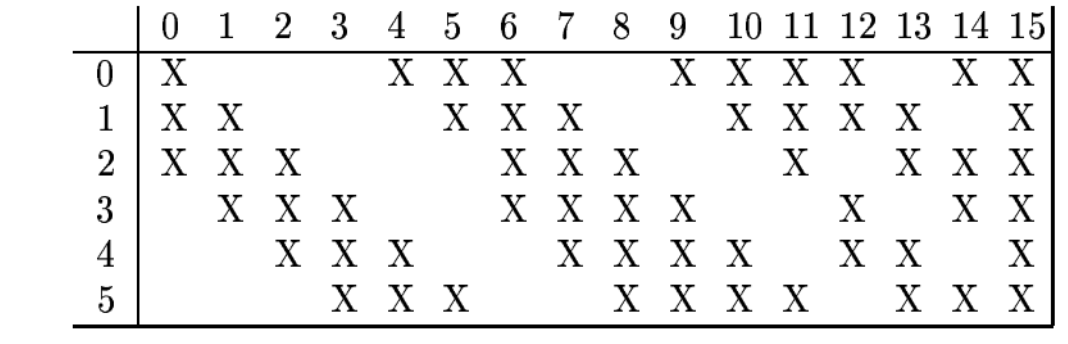
\includegraphics[width=0.65\textwidth]{Figures/connections}
\caption[Connections]{ Each column indicates which feature maps in S2 are combined by the units in a particular feature map of C3. \cite{lenet}}
\label{fig:Lenet Connections}
\end{figure}

Similarly the feature maps at S2 are followed by another convolution and another subsampling layer C3 and S4. The outputs of S2 however are not connected all-to-all to the third convolution instead only the marked slots in the table 1 below shows that only some combinations of the feature maps in S2 are connected to C3. The purpose is to avoid overfitting to the full S2 features by breaking the symmetry and hopefully discovering different feature abstractions from the different set of inputs \cite{lenet}. It also serves to decrease the amount of trainable parameters in the model. 

The convolution stage ( C1  $\rightarrow$ S4 ) is followed by two fully connected layers C5 and F6 of sizes 120 and 84 neurons respectively. Note that the reason C5 is labeled as a convolution layer (even though it performs the role of a fully connected layer) is that if the network were scaled for bigger inputs, the output feature map for C5 would be larger than 1x1. 

The last fully connected layer is fed into the output which is composed of Euclidean Radial Basis (RBF) \cite{chen1991orthogonal}. It computes the euclidean distance between the input vector and a trainable parameter vector (eq.1). The model was trained on a set of 60,000 images and achieved a minimum test-error of 0.7\% competing with all of the other neural network models at the time. Some of the input training images were translated slightly, and rotated by up to $\pm{30^\circ}$ to increase the network’s robustness by making it slightly more translation and rotation invariant. 

Even though the Lenet is outdated and has been replaced by many other neural networks, we choose to this network as a prototype to build our DNN framework due to the simplicity of the implementation. We implement it not for its usefulness but rather more to guide our study into optimizing layer implementations and thinking about methods to improve throughput and achieve pipelining between the layers. 

\subsection{Modern Architectures} 

\subsubsection{AlexNet}

\begin{figure}[h!]
\centering
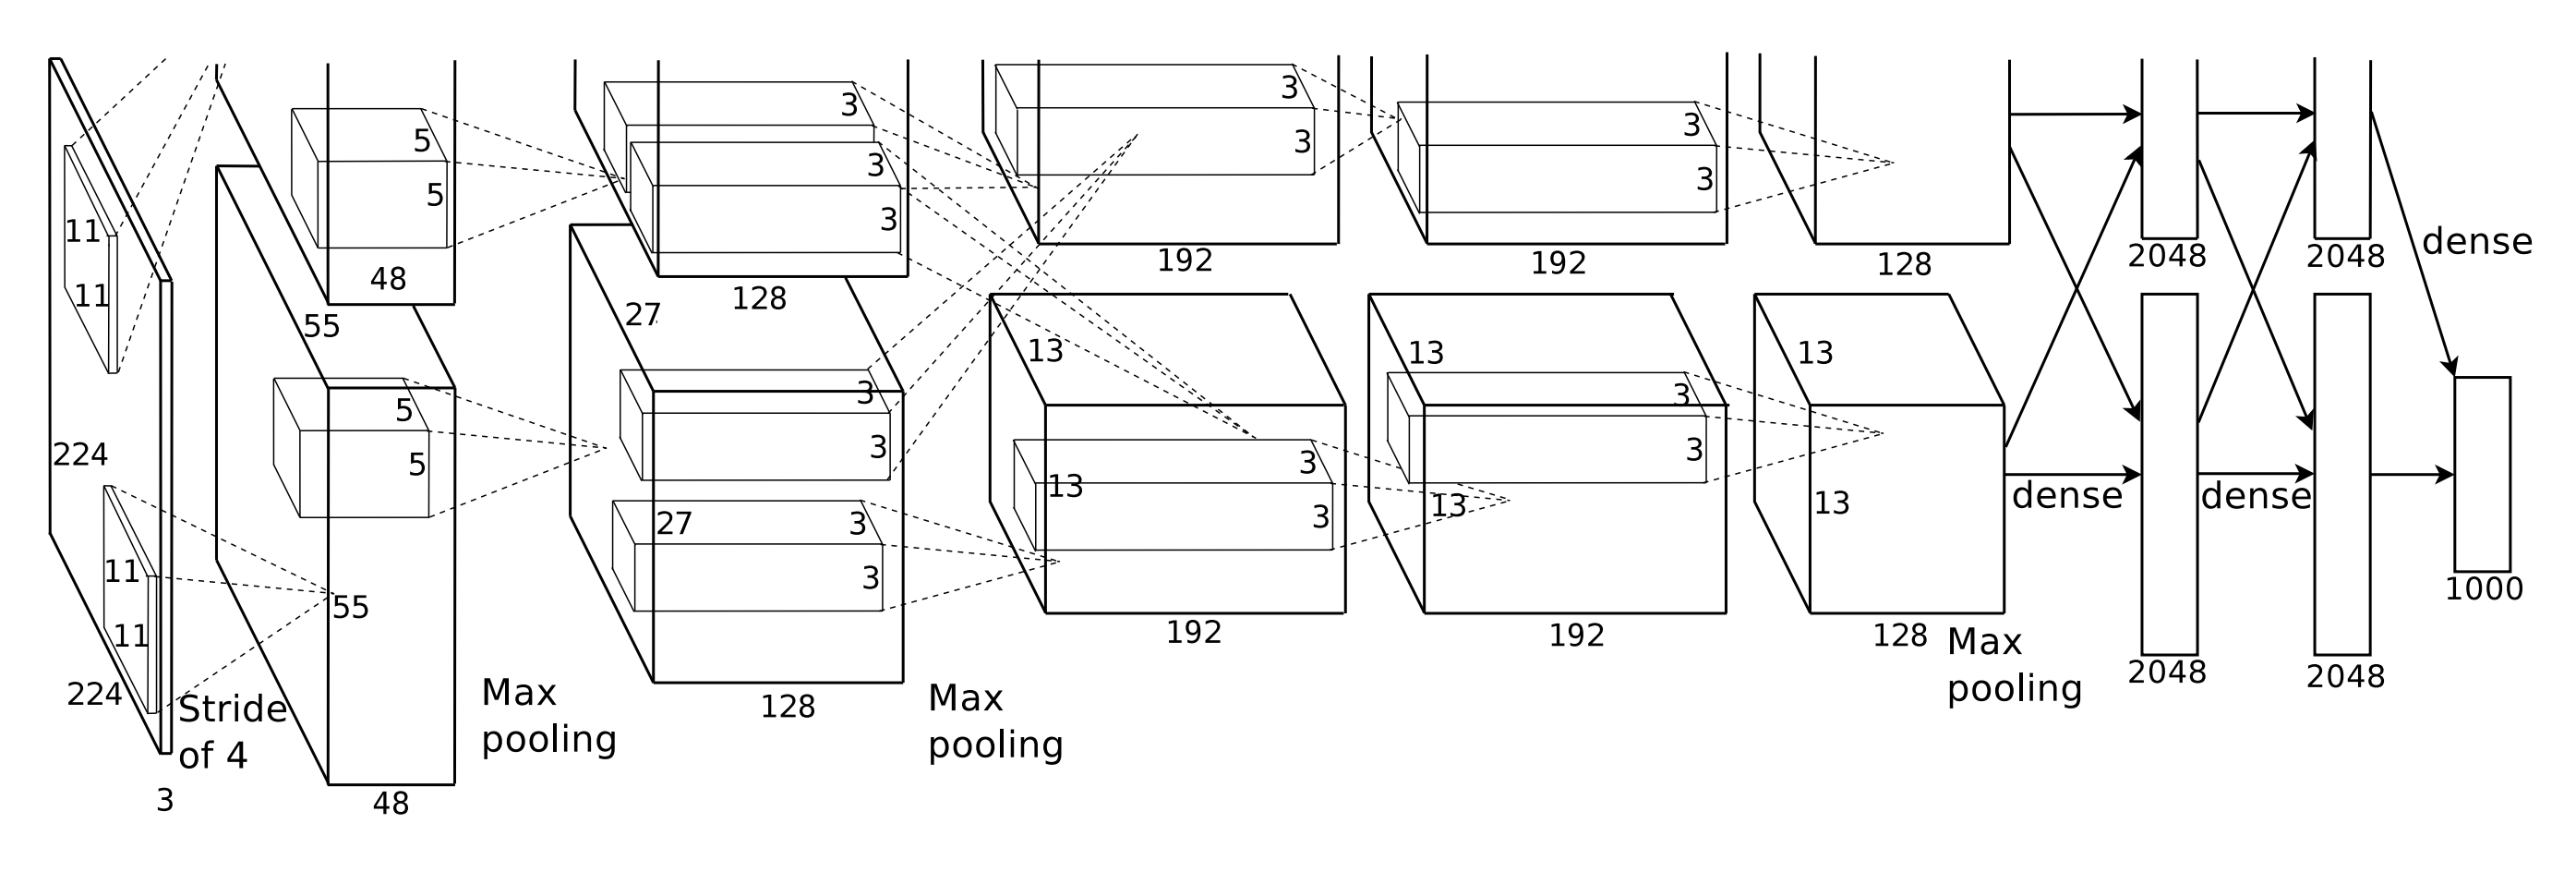
\includegraphics[width=1.0\textwidth]{Figures/alexnet}
\caption[AlexNet]{ Alexnet Architecture  \cite{alexnet}}
\label{fig:AlexNet Architecture}
\end{figure}

AlexNet \cite{alexnet} won the ImageNet Large-scale Image recognition competition in 2012. It follows the Lenet’s approach of staging some convolutional layers back-to-back and then eventually terminating with fully connected layers to perform the classification. It was able to achieve 26.25 top-5 error in the task of classification of three-channeled 224x224 images into 1000 classes. The network was trained on a GPU \cite{alexnet} and used local response normalization layers. In addition to that the authors used dropout which is a technique against overfitting in a network \cite{dropout}. It involves randomly picking out neuron connections and setting them to zero thus decreasing the number of trainable parameters in the model. What also differs from LeNet is the use of Rectified Linear Units (ReLU) activations and maxpooling \cite{alexnet} for the subsampling layers.

\subsubsection{ResNet}

\begin{figure}[h!]
\centering
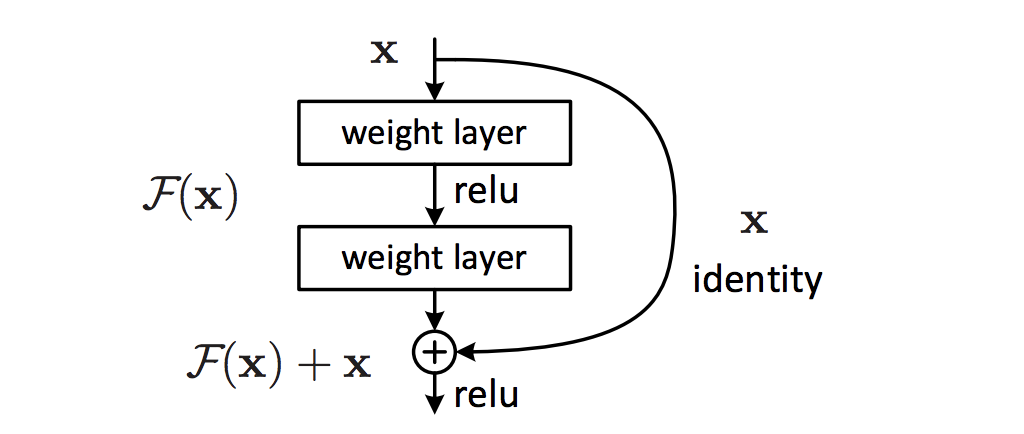
\includegraphics[width=0.7\textwidth]{Figures/residual}
\caption[Residual Learning]{ A basic building block in residual networks showing the identity shortcut  \cite{resnet}}
\label{fig:Residual Learning Basic Block}
\end{figure}

ResNet \cite{resnet} is one of the modern networks that sacrifices breadth for depth. Training deeper network is harder because of a problem discovered by Hochreiter et al. \cite{hochreiter1998vanishing} of vanishing gradients.  The authors of ResNet augment the network with shortcut connections that act as identity layers and enable training with respect to residuals instead of the original input values. Using this trick it was possible to train deeper networks reaching up to more than 150 layers. 

%----------------------------------------------------------------------------------------
\section{Training and Backpropagation}

The above networks all try to achieve the goal of properly approximating a mapping function between the dataset inputs and the given labels. In the example of Lenet, inputs are normalized 28x28 single channels, and the output of the network is a the most probable digit between 0 and 9 that this image represents. Formally described, given an input domain $\mathit{X}$, an output set of labels $\mathit{Y}$, and a set of candidate functions $\mathit{f : X \rightarrow Y}$ belonging to a hypothesis class $\mathit{H}$, we are trying to minimize the loss of mispredicting the correct class. The loss function can be expressed as :
\begin{equation}
L_D(f) = p( f(z) \neq h(z)) 
\end{equation} 
 
 where $\mathit{z}$ is a sample from the dataset $\mathit{D}$,  $\mathit{f(z)}$ is the output prediction and $\mathit{h(z)}$ is the true class or label. In that case training is then formalized as finding the best set of parameters $\mathit{w}$ in our model to minimize this loss function. 
\begin{equation}
 w* = \argmin\limits_{ w \in \mathit{H} } L_D(f_w)
 \end{equation}

Several options exists for sample loss functions as shown in Table \ref{tab:loss}. In regression, a common loss function is the squared error loss. In classification problems, the binary loss can be used. However, for minimization, the loss function should be both continuous and differentiable. To solve this problem, an alternative cross-entropy loss function is introduced for multi-class classification problems as opposed to the binary loss. The output becomes a probability distribution of the input according to the given possible output classes. The cross entropy loss calculates the difference between the predicted distribution and the true distribution into $\mathit{K}$ classes.

\begin{table}[h!]
	\centering
	\begin{tabular}{| l | c | r |}
		 \hline
	Squared loss 	& $l=(f_{w}(z)-h(z))^{2}$  \\ \hline
	Binary loss 	&  $l=\left\{\begin{array}{cl} 0, & \mbox{if }f_{w}(z)=h(z)\\ 1, & \mbox{if }f_{w}(z) \neq h(z) \end{array}\right.  $ \\ \hline
	Cross-entropy loss 	& $l=\sum_{i=1}^{K}f_{w}(z_{i})\log(h(z_{i}))$  \\
	 \hline
	\end{tabular}
\caption{Examples of loss functions}
\label{tab:loss}
\end{table}

\subsubsection{Gradient Descent}


To solve the minimization problem, we can either use evolutionary algorithms inspired by natural processes and meta-heuristics or we can resort to the use of iterative approaches. It is more popular in machine learning to use the iterative gradient descent techniques. In gradient descent, starting from an initial set of weights, we calculate the gradient of the loss function with respect to the weights  $  \frac{\partial L}{\partial w}  $ and iteratively adjust the weights in the direction of the gradient to minimize loss ( $ \eta $ is the learning rate.
\begin{equation}
 w^{t} = w^{t-1} +  \eta \frac{\partial L}{\partial w} 
\end{equation}
The error is back-propagated layer by layer from the output to the input layer by utilizing the chain-rule.
 
 \begin{figure}[h!]
\centering
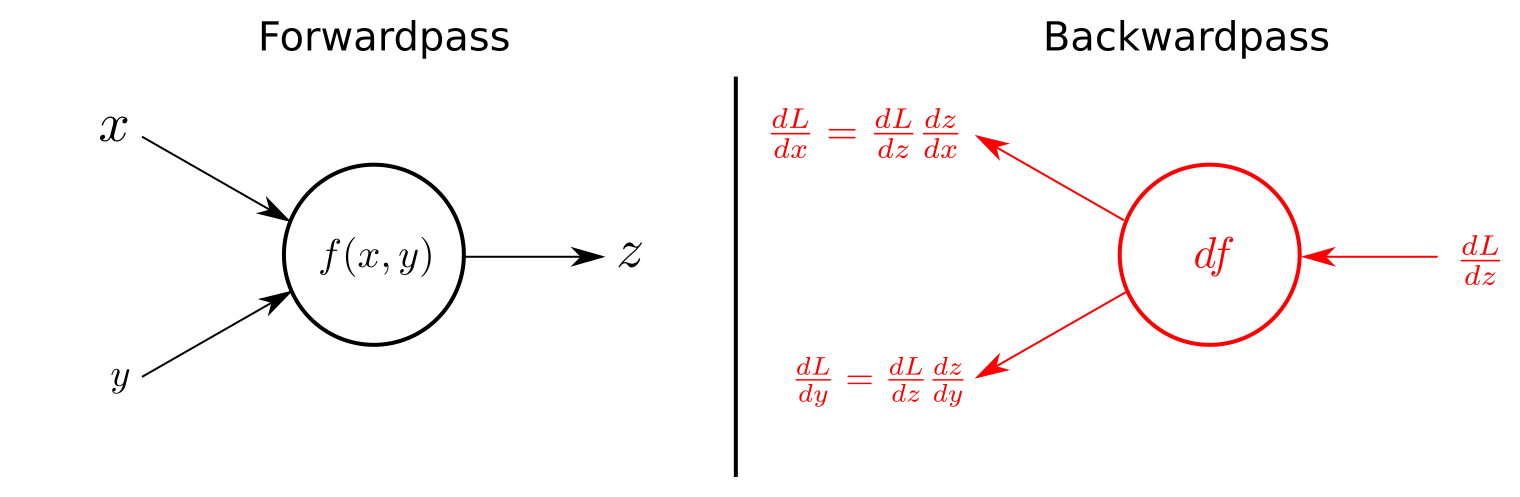
\includegraphics[width=0.9\textwidth]{Figures/backprop}
\caption[Backprop]{ Local Gradient Backpropagation using the Chain Rule Source:\footnotemark} 
\label{fig:Forward and Backward Passs}
\end{figure}
 
\footnotetext{\url{https://kratzert.github.io/2016/02/12/understanding-the-gradient-flow-through-the-batch-normalization-layer.html} Last Accessed: 23/08/2018}
%---Add gradient descent algorithms as pseudo code

%---Compare 3 types of gradient descent
Gradient descent implementations vary depending on how many samples are used to calculate the error. The three main types are batch, stochastic, and mini-batch gradient descent \cite{ruder2016overview}. The different types also exhibit tradeoffs in terms of computations required, frequency of updates, convergence, and stability of the calculated gradient. 

\begin{minipage}{.7\linewidth}
\begin{algorithm}[H]
N = number of training points\;
 \While{not converged}{
  $ w^{t} = w^{t-1} +  \eta \sum_{i=0}^{i=N}{\frac{\partial L}{\partial x_{i}} \frac{\partial x_{i}}{\partial {w} } } $ \;
 }
 \caption{Batch Gradient Descent}
\end{algorithm}
\end{minipage}

In Batch Gradient Descent (BGD), the error is calculated for all of the samples in the training set. After all of the samples have been observed, the error can be backward propagated through the layers and the weights are updated. This complete forward pass and the backward update is called an epoch and usually neural networks are given a fixed set of epochs to train or we keep training until a certain accuracy is achieved. The benefit of using batch gradient descent is that the complete gradient is computationally efficient and presents stable convergence. Stability on the other hand makes it harder to avoid local minima and the minimization problem can easily get stuck in a local minimum. Knowing that the optimization problem of neural networks is riddled with saddle points, we might want to resort to different types of gradient descent. 

\begin{minipage}{.7\linewidth}
\begin{algorithm}[H]
N = number of training points\;
Randomly Shuffle Data Points\;
 \For{i=1, ..., N}{
  $ z \leftarrow x_{i} $ \;
  $ w^{t} = w^{t-1} +  \eta \frac{\partial L}{\partial z} \frac{\partial z}{\partial {w} } $ \;
 }
 \caption{Stochastic Gradient Descent}
\end{algorithm}
\end{minipage}

Stochastic gradient descent (SGD) offers an alternative to calculating the full gradient and passing in the whole dataset. Instead, a random sample is selected from the dataset and forward propagated, the weights are then updated after backpropagating the gradient resulting from this sample. This update technique is less stable than batch gradient descent but it helps in avoiding local minima. It has also been proven that it converges with a rate of  $ \frac{1}{\sqrt{T}}  $ where $ \mathit{t} $ is the iteration number or epoch  for convex functions. SGD demands more computational power due to the frequent updates especially when the training set is large.


\begin{minipage}{.7\linewidth}
\begin{algorithm}[H]
N = number of training points\;
B = batch size\;
 \For{i=1, 1+B, ...N-B+1}{ 
 $ w^{t} = w^{t-1} +  \eta \sum_{j=i}^{j=i+B-1}{\frac{\partial L}{\partial x_{j}} \frac{\partial x_{j}}{\partial {w} } } $ \;
  
 }
 \caption{Mini-batch Gradient Descent}
\end{algorithm}
\end{minipage}

Minibatch gradient descent comes as the middle ground between SGD and BGD and is commonly used in practice. The weight update is viewed only after a mini-batch is forward propagated. Typical batch sizes are 32, 64, 128 (sometimes much larger in the thousands )  as powers of 2 fit the memory requirements of GPU accelerators and memory requirements. This technique balances the robustness of SGD and the stability of BGD. Minibatch introduce another hyperparameter that increases design space and allows for trying out different values to obtain the best test-accuracy.


%----------------------------------------------------------------------------------------
\section{Parallelism in Deep Neural Networks}
As the models grow in size and have more trainable parameters, more data and computational resources are required to properly train the above networks. For that we can speed up the training process of DNNs by exploiting parallelism from different directions. We can distinguish three main types of parallelism \cite{ddl}; data parallelism by parallelizing over the input dimension, model parallelism by tiling computations and running the same layer concurrently on separate cores, and pipeline parallelism which exploiting the pipeline structure of the networks and run the layers concurrently where one layer’s output feeds into the other layer directly. 

\subsection{Data Parallelism}
The structure of the input and intermediate results of convolutional neural networks as multidimensional grids allows us to use this structure and split up the input into several parts that can also be forward propagated concurrently. The training samples in a batch gradient descent algorithm can be calculated separately before the back-propagation step. The bottleneck in this approach appears when we wish to back-propagate the error and all of the errors are averaged to calculate the gradient with respect to the loss function. The paradigm is suitable for a MapReduce model and can easily be parallelized. The only obstacle to this approach is batch normalization layers where synchronization has to occur at every normalization layer. 

\subsection{Model Parallelism}
In this type of parallelism, the neurons in a hidden layer are divided and computed separately. This can decrease the memory requirement for running the network if the model is partitioned but it also adds the overhead of communication between the different parts of the model. For example in an all-to-all connection in fully connected layers, the intermediate results should be shuffled across different computing nodes and synchronized so that the next layer can be computed. Some improvements have been proposed such as adding redundant computations in fully connected layers so that less communication is required\cite{muller1994neural},  but it comes at the expense of more computations. As for convolutional layers, splitting the task of calculating output feature maps across separate processes would induce an overhead of reading the input map of the previous layer multiple times and is thus impractical.

\subsection{Pipeline Parallelism}
This type of parallelism is similar in a sense to both of data and model parallelism. The multiple stages of computations and layers in a DNN can be all active at the same time in a pipeline order. The idea is that different stages can be working on different parts of the pipeline as data is ready from an earlier stage. This is specifically important to the rest of the work as this is a type of parallelism that only FPGA accelerators can benefit from. On such flexible architectures, complex dataflows and pipelines can be programmed. Some implementations have shown that forward propagation and the backward pass computations can be pipelined together \cite{abadi2016tensorflow, collobert2011torch7}. The challenge in this is that as deep neural networks become bigger, they may not fit within a standard FPGA resources. Two solutions can thus be proposed. On one hand, the layers can be combined together and the network can perform the computations, reprogram itself and then compute another combination of layers. Communication in that case can be done by reading and writing intermediate results to global memory. Another solution can be implemented using the OpenCL SDK for Xilinx (Intel has not yet added support for that in high level synthesis) leveraging the power of partially reconfiguring an FPGA while part of it is performing computations.
 
%% Chapter 1

\chapter{Hardware Implementation} % Main chapter title

\label{Chapter3} %

%----------------------------------------------------------------------------------------

\section{LeNet Pilot} \label{lenetpilot}

The main contribution in this work is in the form of a framework for the development and optimization of deep neural network operators on an FPGA. We use the Lenet \cite{lenet} model, knowing that it is outdated and outperformed by many other network architectures discussed before, due to its simplicity and as a pilot to test our framework. The simple network allows us to implement four different types of layers ( convolution, maxpooling, fully connected layers, and softmax). We also implement the backward propagation operators for all of the above layers.  We use LeNet to guide the numerous optimizations we perform on each layers separately and on the combination of the layers into a pipeline as well. We implement a modern variant of Lenet which only differs slightly from the original one. The first convolution in our model contains 10 feature maps as opposed to 6 in the original lenet\ref{fig:Lenet-5}, the second convolution outputs 20 feature maps as opposed to 15 feature maps. This adds more trainable parameters and thus we hope to use most of the MNIST dataset for training. For the sub-sampling layers we replace the average pooling operation by the maxpooling operation. We also use ReLU activation functions as opposed to the sigmoid as it has a lighter hardware implementaion and it has shown better results than the sigmoid in practice \cite{alexnet}. In the following sections we go more in detail about the implementation of the operators using OpenCL. 

\begin{table}[]
\centering
\begin{tabular}{ll}
\hline
\multicolumn{1}{|l|}{\textbf{Layer}} & \multicolumn{1}{l|}{ \textbf{No. Parameters}} \\ \hline
\multicolumn{1}{|l|}{C1}    & \multicolumn{1}{l|}{260}                            \\ \hline
\multicolumn{1}{|l|}{C2}    & \multicolumn{1}{l|}{5,020}                          \\ \hline
\multicolumn{1}{|l|}{C5}    & \multicolumn{1}{l|}{117,720}                        \\ \hline
\multicolumn{1}{|l|}{F6}    & \multicolumn{1}{l|}{10,164}                        \\ \hline
\multicolumn{1}{|l|}{\textbf{Total}}    & \multicolumn{1}{l|}{133,164}                        \\ \hline
\end{tabular}
\label{tab:custom-lenet}        
\caption{Number of Trainable Parameters for Custom LeNet Implementation}             
\end{table}


\section{Layer Implementations}

\subsection{Convolution Layer}

The fundamental operation in Convolutional Neural Networks is the convolution operation. This layer takes as input a multidimensional grid and extracts output feature maps by sliding a window of weights. The filter weights and biases are trainable by gradient descent. An output feature map pixel $ \mathit{y_{i}} $ is obtained by passing a filter of size $ K_{h}xK_{w} $ over an input feature $ \mathit{x_{i}} $ with $ \mathit{CH_{in}} $ input channels.
\begin{equation}
 y_{i} = relu(\sum_{c=0}^{c=CH_{in}} \sum_{h=0}^{h=K_{H}} \sum_{w=0}^{K_{w}} w_{i,c,h,w} * x_{c,h,w}  + bias_i ) 
\label{eqn:summat}
\end{equation}
The nested loop structure lends itself easily for parallelization.  We will discuss three different implementations for this layer and compare tradeoffs that can be used by the user 

\subsubsection{Simple Implementation with Unrolling} \label{simpleimpl}

With the help of high level synthesis, we can write a C-like implementation and analyze the performance. Assuming the kernel is pipelined we will require $ batch size * Img_h * Img_w * K_h * K_w * CH_{in} * CH_{out}  $ cycles theoretically to complete the convolution. To speed up the naive implementation we perform some optimizations:

\begin{itemize}
\item
\textbf{Unroll over filter computation}: Calculating each pixel in the output feature maps requires $ K_h * K_w * CH_{in} $ multiplications. As our filter sizes are small, we can unroll over the filter dimensions. By unrolling we are effectively parallelizing the algorithm by $ \mathit{25x} $ ( since in our case $ K_h = 5, K_w=5 $ ) . However, we choose to unroll over the input channels and the width of the kernel only. We choose input channels as opposed to only the kernel dimensions due to our memory layout because we stripe the input and  output feature maps by channels as the lowest rank dimension. This increases memory performance by performing batch aligned memory reads. 

\item
\textbf{Buffer the coefficients}: During the forward pass, the filter coefficients, will be read multiple times.  For that, we can reduce the amount of memory reads and buffer the coefficients in low-power and fast registers. This uses space on the board but allows us to access coefficients for a relatively cheaper cost.
\end{itemize}

Summations inside loops, such as in \ref{eqn:summat} can introduce memory dependencies as the result of the next iteration depends on a previous one. Memory dependencies get worse with unrolling factors as the critical path is increased. We carefully transfer the memory dependencies to local memory on the FPGA (discussed in more detail in \ref{loopdep} ) and achieve an ideal iteration index (ii) = 1. Therefore, the theoretical number of cycles for a convolution is expressed as 
\begin{equation}
Latency (L)  \approx ii * batch size * Img_h * Img_w * CH_{out} * K_h  \; cycles
\end{equation}

\lstinputlisting[style=CStyle, caption={code snippet from simple convolution}]{code/convPretty.c}


\subsubsection{Sliding Buffer Implementation} \label{slidingimpl}

In the simple implementation, we buffered the coefficients in low-cost local registers to avoid having to read the coefficients multiple times from memory. We also notice that when the convolution window slides with a stride of 1 step, there will be also values in the input feature map that are re-used. For that, we implement a sliding window that contain's all previously seen values as long as they can still be useful. Our implementation is similar to what is describe by Zohouri et. al \cite{2018combined}. The shift-register holds the input values and multiple taps allow for accessing the desired values in the sliding window. The intel offline compiler performs optimizations like replicating RAM blocks to allow for simulataneous access. For that, only few compiler directives should be specified to make this implementation work \ref{shiftinf}. This implementations is also an example of how we can trade local storage to minimize bandwidth. We also carry over the optimization done in the simple implementation.

\begin{figure}[h]
\centering
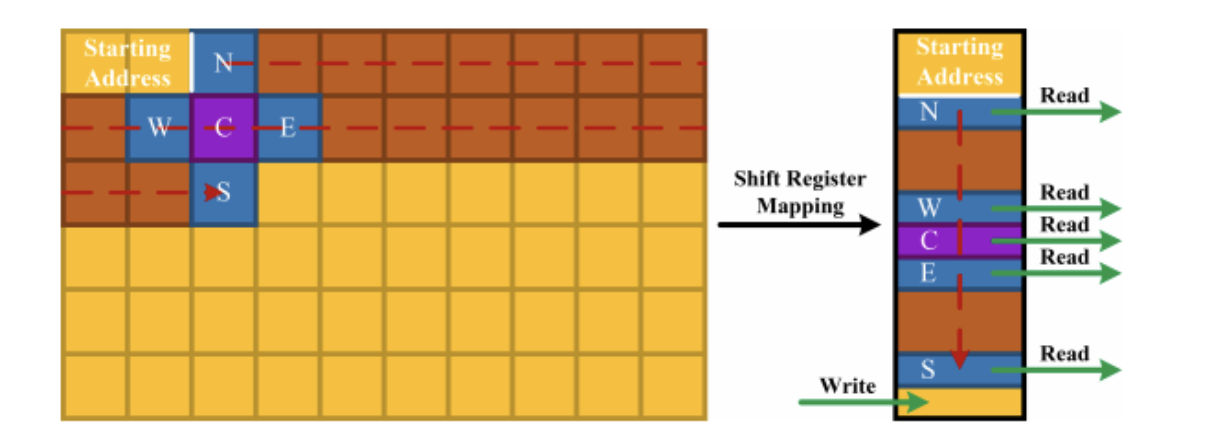
\includegraphics[width=0.6\textwidth]{Figures/slidingbuffer}
\decoRule
\caption[Sliding Buffer]{ Sliding Buffer Visualization. Source: \cite{2018combined}}
\label{fig:sliding buffer}
\end{figure}

\begin{figure}[h]
\centering
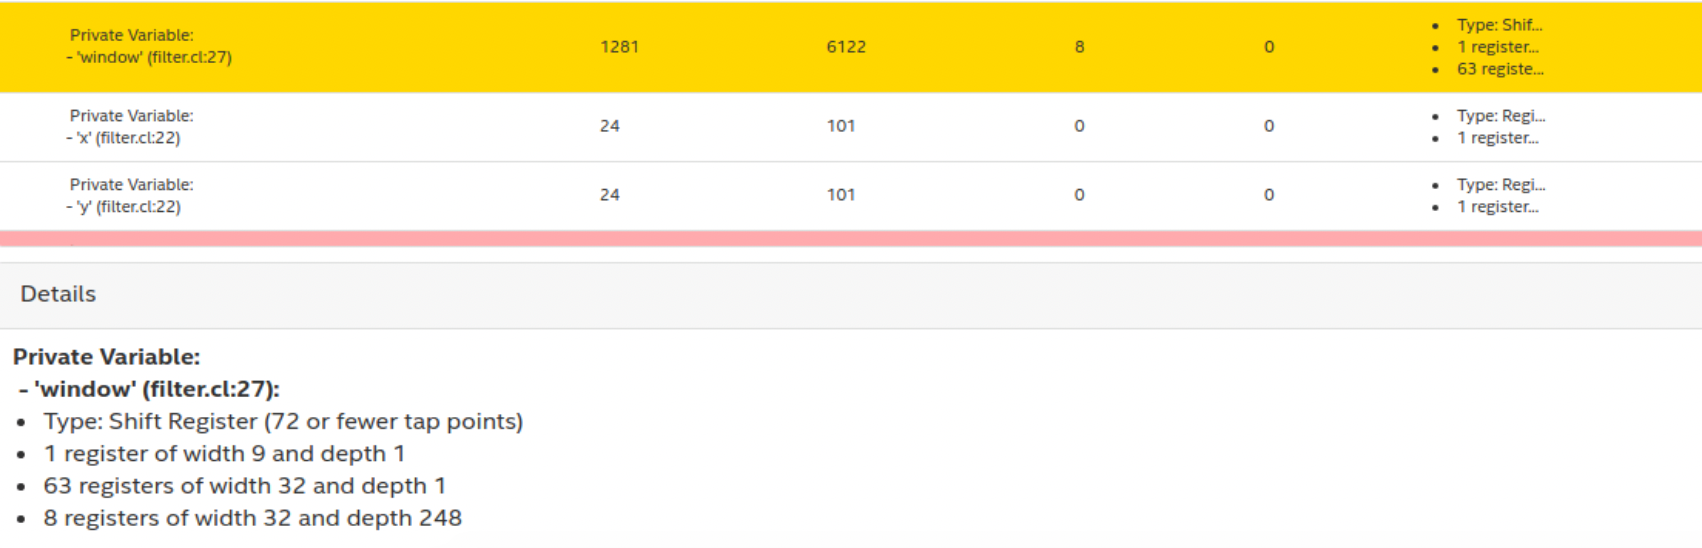
\includegraphics[width=1.0\textwidth]{Figures/shiftregister}
\decoRule
\caption[Shift Register]{ Sliding 'window' variable is inferred as a shift-register by the OpenCL compiler }
\label{fig:shiftregister}
\end{figure}

This implementation proves useful if data is provided in a streamlined fashion. The sliding buffer reads data sequentially and is more suitable for non-blocking dataflow computations.
\newline
\textbf{Limitations}
\newline
One of the limitations this implementation is that we quickly run out of buffer space as the dimensions of the problem grow larger. The sliding buffer size grows linearly with the above parameters: $ CH_{in}, Img_{w}, K_h, K_w $. For our application in a network as small as the Lenet, we do not worry about this problem. The solution to scaling the sliding buffer implementation is to utilize spatial blocking and tile the input into blocks and perform the computations in these tiles separately \cite{2018combined}.

\subsubsection{Row-stationary Implementation} \label{rowimpl}

\begin{figure}[h]
\centering
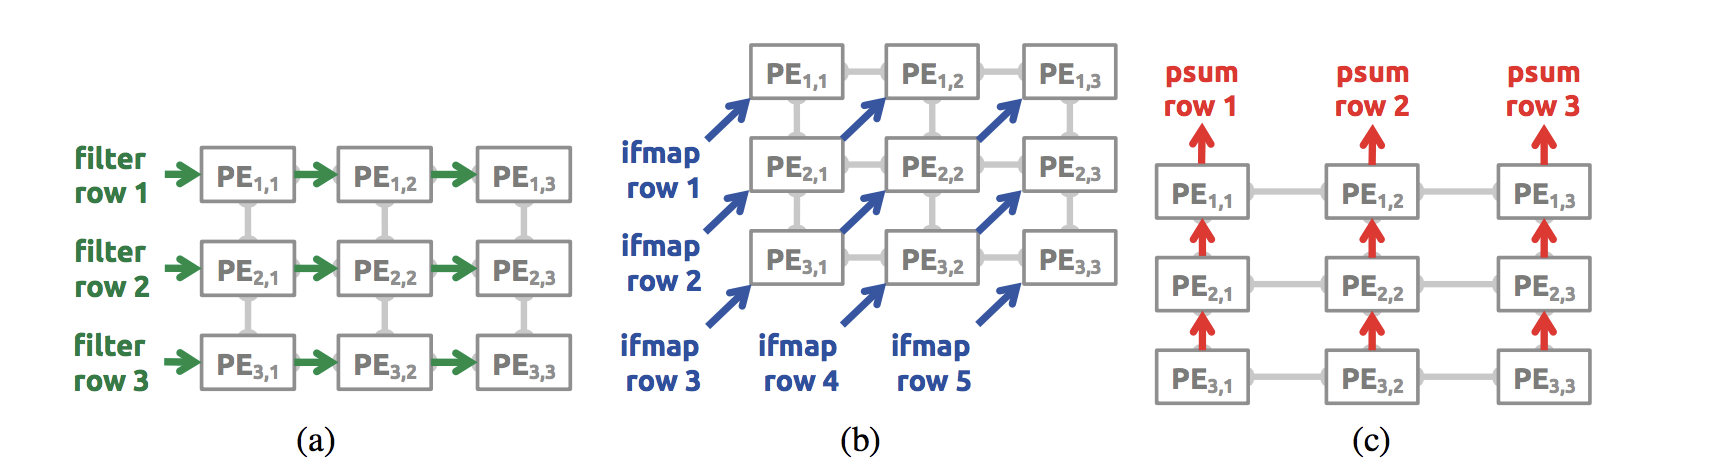
\includegraphics[width=1.0\textwidth]{Figures/eyeriss}
\decoRule
\caption[Data Re-use in Eyeriss]{ Datar re-use across processing elements in Eyeriss. Source: \cite{eyeriss}}
\label{fig:eyeriss}
\end{figure}

\begin{figure}[h]
\centering
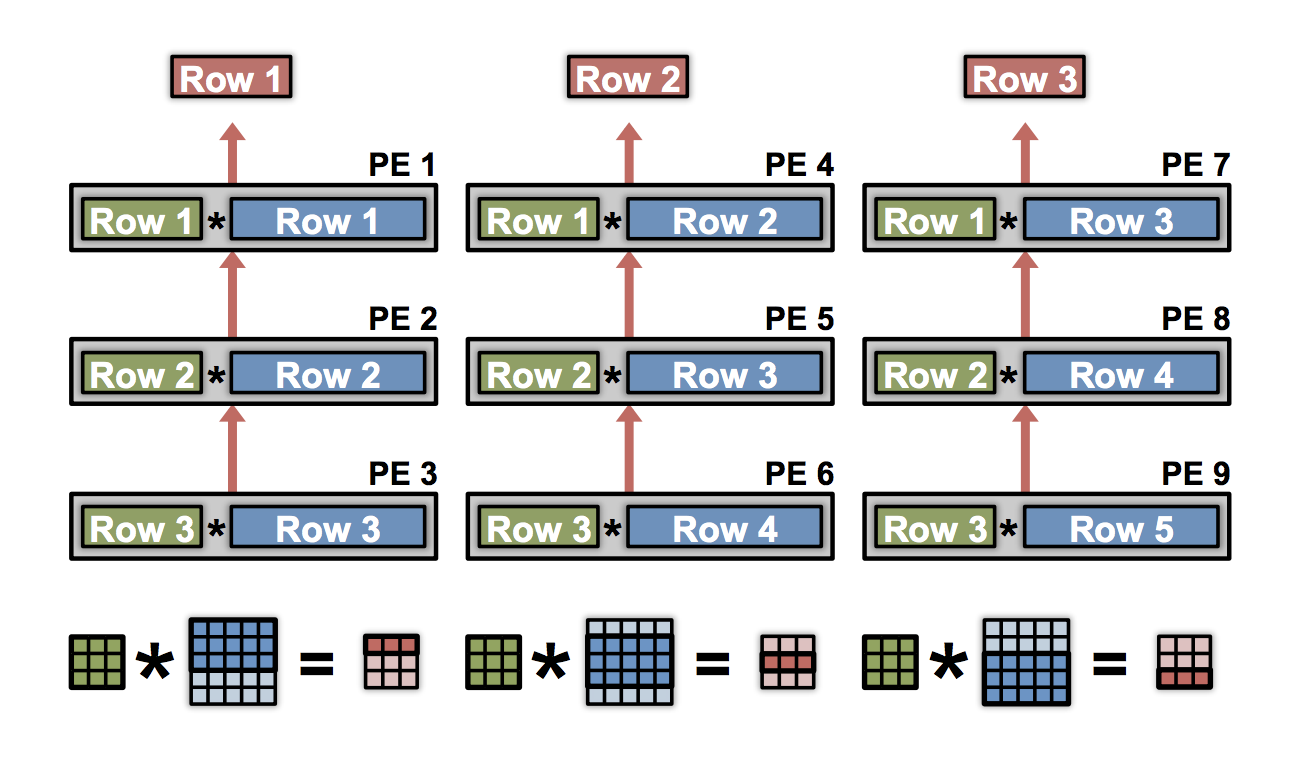
\includegraphics[width=0.6\textwidth]{Figures/eyeriss2}
\decoRule
\caption[2D Spatial Convolution]{ 2D spatial convolution with a grid of processing elements (Eyeriss). Source: \cite{sze2017efficient}}
\label{fig:eyeriss2}
\end{figure}

This approach was suggested by Chen. et. al \cite{eyeriss} and it presents a way of reusing both filter weights and input feature maps. The technique requires a set of replicated processing unit. In the simple case of 3x3 filters we can instantiate 9 processing elements (PEs) each holding one of the 3x3 filter weights \ref{fig:eyeriss}. We implemented a simplified version of this architecture using the Intel SDK’s autorun kernels, which means the kernels do not need to be explicitly invoked and can communicate data to each other using channels ( FIFOs ). Input feature maps are then streamed diagonally (blue \ref{fig:eyeriss}) where they are required for the computation of different output feature map rows. The partial sums are accumulated upwards vertically ( shown in red \ref{fig:eyeriss} ) upwards. 

Advantages of using this is that the size of this grid can be adjusted to best fit the resources available on a specific board. This dataflow performs the theoretical minimum of memory reads required as input fmaps are read once and communicated diagonally to other PUs based on demand. Communication between PEs is done through Intel OpenCL channels which are Intel’s implmentation of FIFOs ( or pipes in OpenCL terms ) and computations are performed asynchronously. Two separate reader and writer kernels handle reading and writing data between global memory and the processing grid. The size of this grid is reconfigurable and the user can instantiate a larger version of this grid. It is independant of the image and filter sizes as we reuse techniques from Eyeriss \cite{eyeriss} such as folding and replication to map different computations onto the same fixed grid.


\subsubsection{Other Implementations}

The below methods were \textbf{not implemented} but it is worth discussing other approaches to performing a convolution. The shared idea is to transform the convolution operation into another form of computation with different properties thus allowing to perform different types of optimizations. 

\textbf{Matrix Multiplication:} One solution to the convolution problem involves transforming the input matrix and incorporating redundant data as in \cite{cudnn}. This transforms the convolution operation into a direct matrix multiplication. The downside of using this is the requirement of either a larger storage for storing the redundant inputs or a very complicated memory access pattern to be implemented \cite{ddl}.

\textbf{Fast-Fourier Transform (FFT):} Another solution is found by transitioning into the Fourier domain and applying a fourier transform on both the filter and the input image \cite{vasilache2014fast}. In the Fourier domain, a convolution becomes again a matrix multiplication. After multiplication of the frequency domain representations of the filter and the input, we use the inverse-fourier transform to obtain the output image. The fourier-transform decreases the complexity of the convolution operation from $ O(N_o^2N_f^2) $ to $ O(N_o^2log_2(N_o) $ where the input image size is $ N_oxN_o$ and the filter size is $ N_fxN_f $ .The tradeoff in this case is less operations on the expense of additional bandwidth and storage requirements. The quality of this transformation and benefits degrade for smaller filters and thus fourier is usally used in the case when large input features and filters are required \cite{sze2017efficient}. 

\textbf{Strassen's Algorithm}\cite{cong2014minimizing}: can reduce the number of multiplications from $O(N^3)$ to $O(N^{2.8})$\cite{sze2017efficient} . The reduced multiplications lower the space requirement as floating point operators require more space than additions but comes at the expense of numerical stability and storage space requirement to hold and propagate intermediate results \cite{sze2017efficient}.

\subsection{Maxpool Layer}

\begin{figure}[h!]
\centering
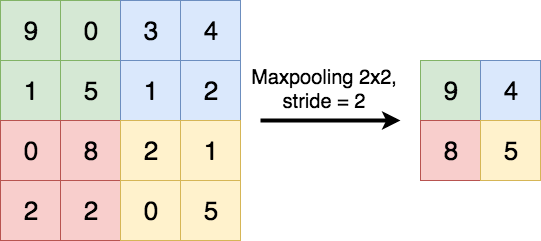
\includegraphics[width=0.5\textwidth]{Figures/maxpool}
\decoRule
\caption[maxpool]{ Maxpooling Operation}
\label{fig:maxpool}
\end{figure}

Convolution layers are usually followed by subsampling layers such as average pooling and maxpooling \cite{lenet}. These operations play a main role in decreasing the size of feature maps in the network and also add to the robustness and also make the network slightly shift-invariant and robust against distortions in the image \cite{alexnet}. Two common subsampling operations are the average pooling where the input values within a certain window are averaged and passed as one output feature map. The second type, which we choose to implement is the maxpooling which passes only the maximum value within a certain window in the input feature map to the output feature map. We developed two different implmentations for the maxpool operation which are the bandiwdth heavy, and streamlined version. 

\textbf{Bandwidth heavy:} the max operation within a certain window can easily be parallelized. In fact the maximum of the four values can be calculated in a single cycle and we can compute the one output pixel in the output feature map at a single clock cycle. Assuming we have sufficient bandwidth we can in fact perform the maxpool reduction to the whole input feature in one cycle however this requires reading the full feature map from memory at once which is impractical. For that, we limit the parallelization to the size of the window. In lenet, it is $ 2x2 $ which gives us a $ 4x $ speedup over the naive implementation of the sequential version of the problem. 

\textbf{Streaming calculation:} As we aim for efficiently pipelining the operators in a convolutional neural networks. We take into consideration the out input feature maps will be streamed in as an input. Therefore to perform the maxpool operation we should buffer in the whole first row and then we can proceed to produce the outputs sequentially. So assuming we are reading our data through an OpenCL channel, the way to fix this is to borrow from the already implemented solution for the sliding buffer convolution. In fact, the maxpool operation iterates over an ifmap as a convolution however in our case the stride size is equal to the filter dimensions $ 2x2 $. We adapt the sliding buffer implementation from the convolution layer to the maxpool layer and use it in our generic maxpool template. 

\subsection{Non-Linearities} 

In between convolution layers and fully connected layers, non-linear functions are applied on the output feature maps. Without non-linear functions, a neural network ( no matter how many layers it consists of ) would behave as a single layer perceptron because summing the layers would give just another linear function. We implement both classical non-linearities such as the sigmoid function and the hyperbolic tangent, in addition to the ReLU function. The ReLU non-linearity  define as $ relu(x)  = max(0, x) $ has proven to increase accuracy \cite{alexnet}, in addition to accelerating training as the derivative can be simply coded as $ relu'(x) = 1 $ if $ (x \geq 0 ) $ else $ 0 $ .  In terms of hardware the relu derivative is simply a MUX wired to constant values of 0 and 1. We implement these operations as a streamlined operation which is pipelined with an $ ii $ of 1.

\subsection{Softmax}

For the output layer we implement the \emph{Softmax} operation. It can be used as a modular output layer for a network that performs multi-class classification such as the LeNet. The operation is defined as follows: 
\begin{equation}
	f(z_j) = \frac{e^{z_j}}{\sum_{k=1}^{K} e^{z_k} } \hspace{1cm}  \mbox{\emph{for j=1,...,K}}
\end{equation}
and it is used to map K outputs to K possible probability values in a categorical distribution. This function highlights the maximum values and suppresses those that are a certain order of magnitude below the maximum value.  Due to the interdependency for normalizing the outputs, the softmax needs to read all output values before it operates, however the operation is unrolled, and since this is the final layer the output of this operation is written directly to memory.

\subsection{Backpropagation}

Backpropagation for all of the layers in the above sections. We summarize all backpropagation kernels in one section for two reasons; the first being that backpropagation operators borrow the same implementation from the forward calculations.i.e backprop of a convolutional layer is also a convolution, and backprop of a fully connected layer is also a matrix multiplication. We believe that the main challenge introduced by implementing backpropagation is that It requires additional buffer space to hold intermediate outputs. For that we are faced with two options:
\begin{itemize}
\item
Replicate writes in the pipeline to global memory and find a way to synchronize forward and backward operations.
\item
Use kernels that read and write to memory and run them sequentially and then eventually run backpropagation.
\end{itemize}

\begin{figure}[h]
\centering
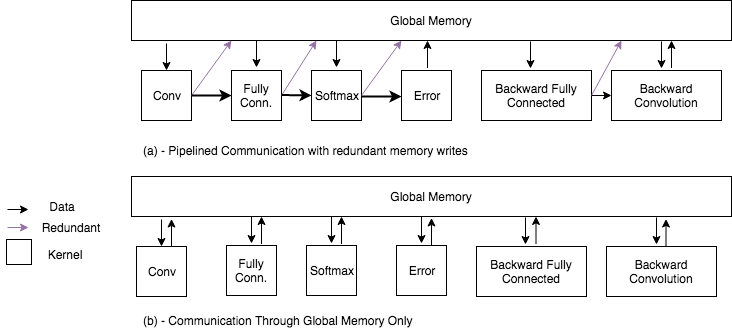
\includegraphics[width=0.9\textwidth]{Figures/comm}
\caption[Types of inter-layer communication]{ Two types of inter-layer communication }
\label{fig:comm}
\end{figure}

We choose to go with option (b) in training neural networks, though not optimal, due to time limit constraints. Our backpropagation algorithm is not pipelined only due to the fact that we need to store intermediate results and this makes it easier as a first prototype for training neural networks on FPGAs. This only impacts performance slightly, because when kernels communicate through memory several parallelization techniques can be performed while sacrificing bandwidth. Also as each kernel runs in a separate timeslot, the whole board bandwidth is available for the single layer which offers us more flexibility in parallelization and making use of the maximum bandwidth. Another thing to note is that profiling kernels is easier and we can better see the time consumed by each kernel and relieve bottlenecks for different operators or architectures 

Backpropagation is the process of propagating an an error back to the network layers in order to adjust the weights. The gradient is propagated backwards in the network based on the chain rule in differential calculus. Several weight update rules ranging from a fixed learning rate to adaptive and momentum-based methods are explored in literature \cite{ddl}. In our implementation we keep the learning rate as an input argument so that it can be configured at runtime by the host program. This allows for flexibility in experimenting with different weight update rules without the need to rebuild the kernel.

The trainable weights are usually initialized to small random values in the range $ (-0.5,0.5) $. In practice, the random weights are then normalized depending on the weight activations used\footnote{\url{https://medium.com/usf-msds/deep-learning-best-practices-1-weight-initialization-14e5c0295b94} Last Accessed: 25/08/2018}. There are also different weight normalization schemes used in practice to mitigate ( but not completely solve ) problems that arise in deeper networks like the vanishing or exploding gradient \cite{hochreiter1998vanishing}. For the ReLu activation, it is common to multiply the random weights by a factor of $ \sqrt{\frac{2}{sizeof(prev. layer)}} $. This initialization is done on the host side and the weights are then transferred to the FPGA in the beginning of the training procedure. 


\begin{figure}[h]
\centering
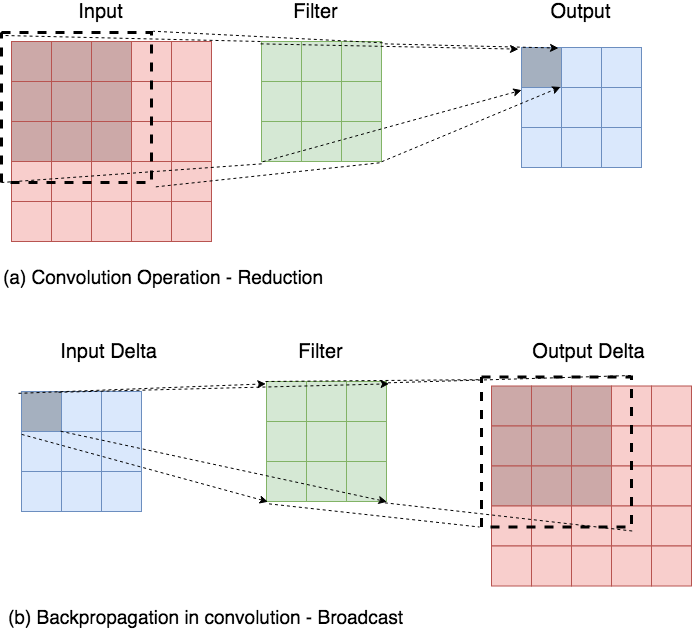
\includegraphics[width=0.6\textwidth]{Figures/convprop}
\caption[Propagation of data in convolution]{ Propagation of data in convolution }
\decoRule
\label{fig:conv}
\end{figure}

\textbf{Convolution Backpropagation:} The backpropagation of a convolution operator is also a convolution. For that we borrow some optimizations performed on the forward convolution such as buffering the coefficients, and unrolling over kernel dimensions. We note the main difference is that in inference phase, a window of dimensions $ K_wxK_h $ is sliding along an input feature map in order to obtain an output feature map. Thus this is more of a \emph{reduction} performed by multiply and accumulation of values in a specific window. In the case of propagating back an error, the input delta ( coming from the output feature map ) is \emph{broadcast} to all of the pixels in the input feature maps ( also show a picture here ). A simple implementation would introduce memory dependencies on calculations, another way is to rearrange dimensions and use local buffering to hold values of the output deltas before writing to memory. The backpropagation kernel we implemented is fully pipelined with $ ii=1 $ and also performs batched weight updates for the filters.

\textbf{Maxpool backpropagation:} For backpropagation through maxpool, we simply pass upstream the error to the input pixel in a certain window with the maximum value. The same implementation from the forward max pooling is used with the addition of passing an output gradient at the maximum as opposed to passing the maximum value downstream. In our case the maxpool does not have any trainable parameter and acts as a multiplexor that passes down the error as it is. 

\textbf{Fully connected backpropagation:} The fully connected layers used for classification contain most of our trainable parameters. In the case of minibatches we use a matrix multiplication technique for both forward and backward propagation of the error. We also try to unroll computation loops to utilize the maximum bandwidth available for this kernel. The backpropagation is a similar inverse computation ( still matrix multiplication)  and the weights are also updated according to a configurable learning rate.

\textbf{Loss}: For the loss function we implemented a cross entropy loss function (\ref{tab:loss}). It measures divergence of the softmax output probabilities ( representing a categorical distribution ) with the target output probabilities as a \emph{one-hot} encoding.

\section{OpenCL Kernel Template Generator}

Many parameters such as sliding window sizes, kernel size, and number of input and output channels should be known at compile time. Each of the discussed layers is parametrized by a specific set of parameters that it takes in as a configuration. For that we created a python tool that instantiates instances  given a kernel template in ‘.cl’ format ( the extension for OpenCL kernels). The idea is to use a configuration file in JSON to customize a specific layer. In conjunction, we used a python library called jinja2\footnote{\url{http://jinja.pocoo.org/docs/2.10/} Last Accessed: 25/08/2018} to instantiate templates.Templating allows us to instantiate multiple versions of the kernel to be used and compiled together for the neural network accelerator.


\begin{figure}[h!]
\centering
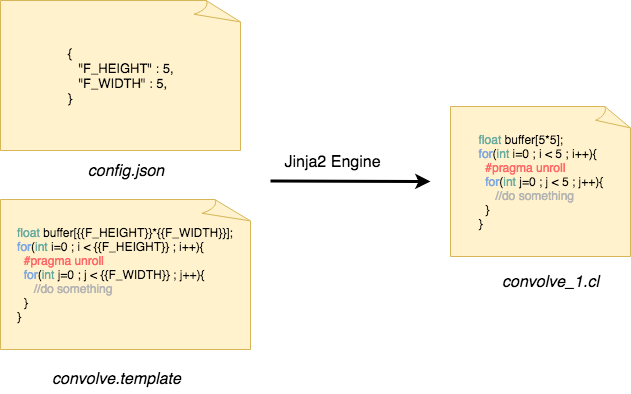
\includegraphics[width=0.9\textwidth]{Figures/jinja}
\decoRule
\caption[Templating Kernels]{ Templating Kernels }
\label{fig:jinja}
\end{figure}

\begin{figure}[h!]
\centering
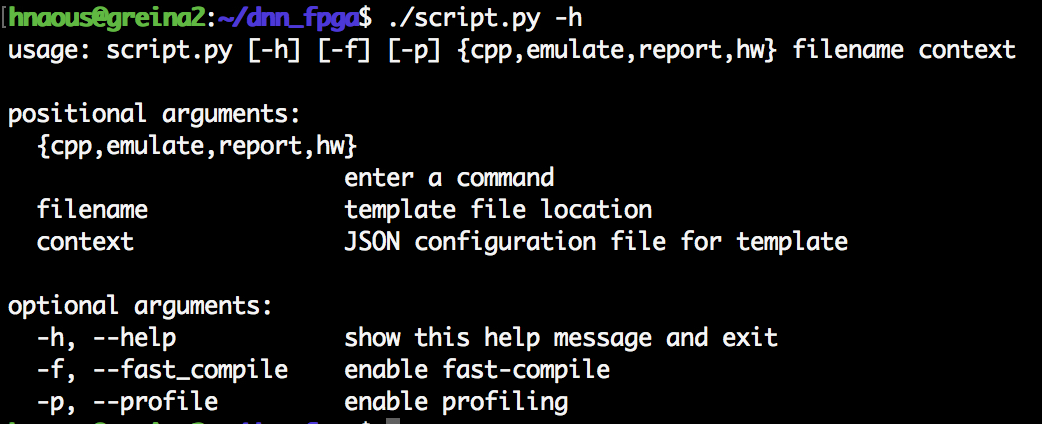
\includegraphics[width=0.7\textwidth]{Figures/usage}
\decoRule
\caption[Tempate Generator Usage]{ OpenCL Template Generator Usage }
\label{fig:usage}
\end{figure}

The basic usage is exposed through the interface shown in \ref{fig:usage}. The Python tool allows the user to also perform additional tasks on the generated kernel such as generating the performance report, compiling for emulation, compiling for hardware, and compiling the kernel as a as a C++ application using gcc. We discuss the use of compiling   as a C++ application in section 5(REF HERE). This type of compilation differs from the traditional workflow suggested by Intel as we have extended the emulation framework of kernels and use C++ to perform unit testing and verifying correctness of the operators. This rids us from the responsibility of creating a host program that interfaces with the kernel and from a lot of overhead code in managing the device buffers just for the sake of verification. 
As for the additional functions such as generating report, and compiling for hardware, the additional value provided by the tool is that it supports instantiating multiple templates at the same time and combining them in a single report or a single binary. All of the kernel implementations discussed in \ref{Chapter3} are designed as templates and the generator tool is used for instantiation, and interaction with the Intel compiler to perform different types of analysis.

\section{Integration with Deep500}

Deep500\footnote{\url{https://github.com/deep500} Last Accessed 25/08/2018} is a library developed internally in the Scalable and Parallel Computing Lab at ETH to aid in the process of developing custom backends for computational graphs. It enables the extension of operators, verification, network optimization, and acts as a distributed learning framework for deep neural network models. The networks are expressed in ONNX\footnote{\url{https://github.com/onnx/onnx} Last Accessed : 25/08/2018 } format. ONNX is an open source format to represent computational graphs ( specifically deep neural networks ). It allows the interoperability between different deep learning frameworks such as torch\cite{torch} and tensorflow\cite{tensorflow} and the exchange of models and parameters in between those frameworks for performing optimizations, training, and inference. 

\begin{figure}[h!]
\centering
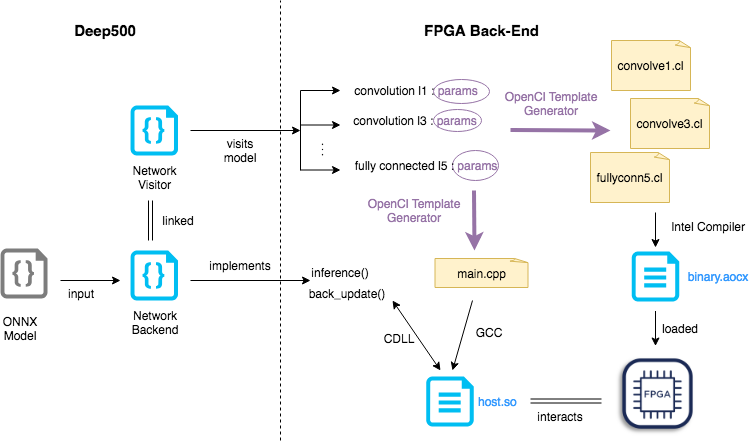
\includegraphics[width=1.0\textwidth]{Figures/integration}
\decoRule
\caption[Intergration with Deep500 Diagram]{ Custom FPGA Back-End for ONNX Models }
\label{fig:integration}
\end{figure}

The Deep500 library provides us with an extendable visitor interface to implement each of the operators required for a given onnx model. For example in our network, the operations we implement are convolution, maxpooling, relu, and gemm ( generalized matrix multiplication ). The Deep500 library traverses the model’s operations using a NetworkVisitor class. We extend the visitor class to implement all of the mentioned operations. Each visit to a node in the graph provides the parameters and input shapes required for implementing this node's operation. We use those parameters to instantiate an OpenCL kernel using the template generator we created. With the \emph{.cl} files available, we are able to transform an ONNX model into a group of inter-related OpenCL kernels that can be built for hardware \ref{fig:integration}. From there we can use again the tool to view the area utilization report, emulate the kernel, and perform additional unit tests on each of the operations.
To enable training and inference using the kernels and built CL files, we require a host program running on the CPU that interacts with the above kernels. The host program is in C++ and has to be customized for the computational graph it runs. For that we choose to template the host program also using  \emph{jinja2}. In addition, we also use the operation parameters to be able to generate a suitable host program.  
\emph{jinja2} allows us to use nested JSON configurations and arrays in order to generate the host program. The host program performs the following operations : setting up opencl environment, passing data between the host program and the FPGA's global memory buffer, and enqueuing kernels to be executed on the FPGA.

For the accelerator backend to work it should communicate with the templated host program, so after instantiating the host program, we compile it as a shared object \emph{'host.so'}. This allows us to use python’s CDLL library to create a handle to the C++ program. The forward and backward propagation functions are exposed externally to CDLL and we can easily pass down coefficients and inputs to the host program,which executes and returns the results.

The added value and end result of this work is given an ONNX model we can create and compile the relevant FPGA binaries by using Deep500 to traverse the graph. We are also able to instantiate and compile a controller host program, and interact with this host program to train a neural network. The benefit also extends to other popular DNN frameworks where models can be exported to onnx. For example the pytorch library offers the option of exporting torch models to onnx, the implementation offers the ability to interact with this tool and train other networks on an FPGA. It is also worth mentioning that  Deep500 allows us to perform unit-tests to verify each of the implemented operations on the FPGA.

%-----------------------------

%% Chapter 4

\chapter{Experiments and Results} % Main chapter title

\label{Chapter4} %

In this chapter, we describe the experiments we ran to verify the functionality of the proposed framework. We also compare different the different implementation alternatives taking kernel execution time as our main metric. All of our experiments are run on the Nallatech 510T Compute Accelerator card which contains an Alterra Arria 10 1150 GX FPGA. Our kernels are compiled with the Intel OpenCL SDK with Quartus 17.1. The host program is compiled with gcc v.7.2.0. All of the tools that support the development workflow were tested using Python 3.6.5. 
The model we use for training and inference is the LeNet discussed in section \ref{lenetpilot}.


%----------------------------------------------------------------------------------------
\section{Convolution Implementations}

\begin{table}[]
\centering
\begin{tabular}{|l|l|}
\hline
\textbf{Parameter}    & \textbf{Value} \\ \hline
Image                 & 100x100        \\ \hline
Filter                & 3x3            \\ \hline
Input/Output Channels & 1              \\ \hline
\end{tabular}
\caption{Configuration for the Part I Test Case}
\label{tab:partoneconfig}
\end{table}

\subsection{Part I : Simple Example} \label{testone}
In this section, we compare the different convolution implementations. Those are the simple implementation, sliding buffer, and row-stationary \ref{rowimpl}. The parameters are shown in Table \ref{tab:partoneconfig}. 

\begin{figure}[h]
\centering
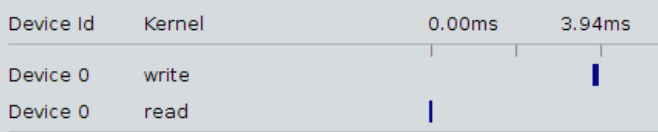
\includegraphics[width=0.7\textwidth]{Figures/profilerow}
\decoRule
\caption[profilerow]{ Dynamic Profiling result for row-stationary Implementation}
\label{fig:rowstatp}
\end{figure}

\begin{table}[]
\centering
\begin{tabular}{|l|c|c|}
\hline
\textbf{Implementation}        & \multicolumn{1}{l|}{\textbf{Execution Time (ms)}} & \multicolumn{1}{l|}{Frequency (MHz)} \\ \hline
\textit{Simple Implementation} & 0.15                                              & 256.1                                \\ \hline
\textit{Sliding Buffer}        & 0.09                                              & 252.8                                \\ \hline
\textit{Row Stationary}        & 3.94                                              & 184.4                                \\ \hline
\end{tabular}
\caption{Results of Part I Test}
\label{tab:resultpartone}
\end{table}

The profiling results and operating frequency of the board for each of the implementations is shown in table \ref{tab:resultpartone}. In the case of the row-stationary implementation, the compute array of processing elements are \emph{autorun} kernels. Therefore they are considered to be running the whole time during execution and will not be caught by the Intel Dynamic Profiler. To approximate the time consumed we take the time difference between the reader and writer kernels that communicate with the grid as the execution time.
Unsurprisingly, the row-stationary implementation is the slowest in a small example. One reason is a low operating frequency due to a long critical path of execution. Another reason is the synchronization and communication overhead between the processing elements in the processing grid. We see also that the sliding buffer has the best performance in the case of a single large image which also makes sense. In the next section we abandon the row-stationary implementation and test the two other kernels in a real-case scenario.


\subsection{Part II : Performance in a Real-Case} 

In \ref{testone} we used a very simple two dimensional convolution to benchmark three different convolution operators. Our row-stationary implementation doesn't support a real-case convolution with multiple input and output channels. For that we compare the two other implementations ( sliding buffer, and optimized implementation \ref{slidingimpl}) configured for a large batch of size of $ 2048 $ and for a convolution requiring multiple input and output channels. This allows us to better compare both operators and to choose which one is more suitable for the LeNet model.

\begin{table}[]
\centering
\begin{tabular}{|l|l|}
\hline
\textbf{Parameter} & \textbf{Value} \\ \hline
Image              & 100x20          \\ \hline
Filter             & 5x5            \\ \hline
Input Channels     & 2             \\ \hline
Output Channels    & 6             \\ \hline
Batch Size         & 2048           \\ \hline
\end{tabular}
\caption{Configuration for Part II Test}
\label{tab:l3params}
\end{table}

\begin{table}[]
\begin{tabular}{|l|l|l|l|l|}
\hline
\textbf{Implementation}     & \textbf{Total Time (s)} & \textbf{Frequency (MHz)} & \textbf{RAMS} & \textbf{DSP} \\ \hline
\textit{Simple Convolution} & 5.37                    & 232.7                    & 85            & 4            \\ \hline
\textit{Sliding Buffer}     & 3.53                    & 65.1                     & 116           & 51           \\ \hline
\end{tabular}
\caption{Simulation Results of Different Convolution Implementations }
\label{tab:resultparttw}
\end{table}

The results are shown in Table \ref{tab:resultparttw}. The sliding buffer is faster in practice, however it comes at the expense of more resources and a lower operating frequency. This may be feasible if we only implement the convolution operation, however in the context of a neural network, we chose the first implementation as we wish to fit more network layers in the same binary. The compiled version of the simple implementation differs from that in reference section as we have removed unrolling factors to lower the resource utilization even more. We have found that kernels with resource utilization >50\% take more than 12 hours to compile and we were unable to run the full compilations without timeouts, memory limits exceeded, and placement errors. 

The results are fully pipelined for the batch of images and conform to the theoretical estimate for performance. As compute time for the convolution diminishes the effect of buffering kernel coefficients, we estimate the performance taking into consideration only the main computation loop. For the simple implementation, the calculation is as follows : \newline Number of cycles = batch size * input ch * output ch * img height * img width * filter height * filter width  = $2048 * 2 * 6 * 100 * 20 * 5 * 5 $ = 1,228,800,000 cycles. 

The frequency of operation is $232.7$ MHz, so we can estimate the time to be 5.28 seconds.
\begin{equation}
 Total Time = \frac{Number of cycles}{Frequency} = \frac{1,288,800,000}{232,700,000}  \approx 5.28 sec
\end{equation}
This theoretical calculation matches the experimental results. The same calculation can be performed to the case of the sliding buffer implementation. We note that unrolling factors in the sliding buffer reduce the number of cycles, however this is matched by a lower operating frequency as well.




%----------------------------------------------------------------------------------------
\section{Pipelined vs. Non-Pipelined Inference}

In this example we study the effect of pipelining on the inference phase of the neural network. We test both a pipelined implementation of LeNet \ref{lenetpilot} where kernels are connected by Intel OpenCL Channels and the kernels follow a sliding buffer/streamlined implementation. We also test a non-pipelined version shown in \ref{fig:comm}, where the operators are run sequentially, communicate through global memory, and exhibit different types of parallelism. The batch size is configurable at run-time, so we test the time it takes for the inference of a single image and the time for a batch of 2048 images. 

The results are that the pipelined version is effectively faster than the non-pipelined version during inference. Fig. \ref{fig:pipesingle} shows the dynamic profiler results. We note that the kernels were enqueued into separate queues and also in reverse order in the host program. This is why it seems that the softmax kernel has been running the longest, but effectively it only runs after all of the layers have been completed. We noticed that running the kernels in the order that they are supposed to execute introduced latencies due to context switching and the overhead of enqueuing the tasks from the host-side, so this reverse order gives a more accurate representation of effective time taken for inference. 

The kernels communicate through channels so we are sure that they are synchronized and the results are verified for correctness by using a LeNet CPU implementation configured with the same weights. The kernel also \emph{effectively} starts running after the reader kernel starts (which is at 0.3 ms from the initial start time because it is the last to be launched and all other layers depend on its input). 

The estimation is further verified by running the pipeline to classify a set of 2048 images and the total time taken in that case is 6.12 seconds. A simple calculation in \ref{eqn:check} shows that the theoretical results agree with the experimental results. The dynamic profiler result in \ref{fig:pipebatch} shows that all layers are being effectively utilized in case of batch image inference. 
\begin{equation}
\text{Total time = time for single image * batch size} = 0.03 * 2048 \approx 6.14\text{ seconds}
\label{eqn:check}
\end{equation}

As for the non-pipelined version, we see in \ref{fig:nonpipesingle} that in the case of inference for a single image,  the total time taken for inference is 21.53 milliseconds. Moreover, the effective time by summing up the individual kernel execution times is much less. The reason for the delay in launching kernels is mainly synchronization constructs by calling \emph{clFinish(queue)} in between kernel launches. Summing up individual kernel times leads to an effective execution time of 5.4 milliseconds. This is still significantly slower than the pipelined implementation. For inference of the batch, the effect of synchronization is minimized and we find that the total time of 11.15 seconds meets the theoretical results \ref{eqn:effect}.

\begin{equation}
\begin{array}{l}

\text{Batch Execution time = batch size * effective time one image} \\
  \text{        } = 2048 * 0.054 sec \approx 11.05 sec
\end{array}
\label{eqn:effect}
\end{equation}


\begin{table}[]
\begin{tabular}{|l|l|l|}
\hline
Implementation               & \textbf{Single Image (Effective)} & \textbf{Batch of 2048 Images} \\ \hline
\textit{Pipelined LeNet}     & 0.0033 ( 0.003 )                 & 6.12                          \\ \hline
\textit{Non-Pipelined Lenet} & 0.021 ( 0.0054 )                  & 11.15                         \\ \hline
\end{tabular}
\caption{Inference time for pipelined and non-pipelined implementations of Lenet in seconds. }
\label{tab:resultinf}
\end{table}

\begin{figure}[h!]
\centering
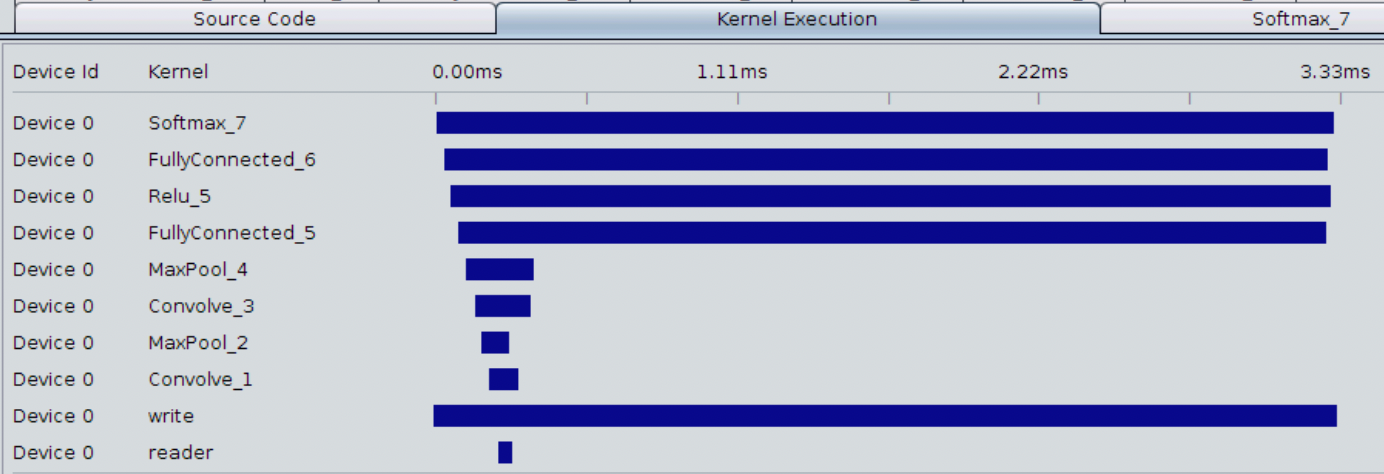
\includegraphics[width=0.85\textwidth]{Figures/pipesingle}
\decoRule
\caption[pipesingle]{ Execution time for inference of a single image (pipelined)}
\label{fig:pipesingle}
\end{figure}

\begin{figure}[h!]
\centering
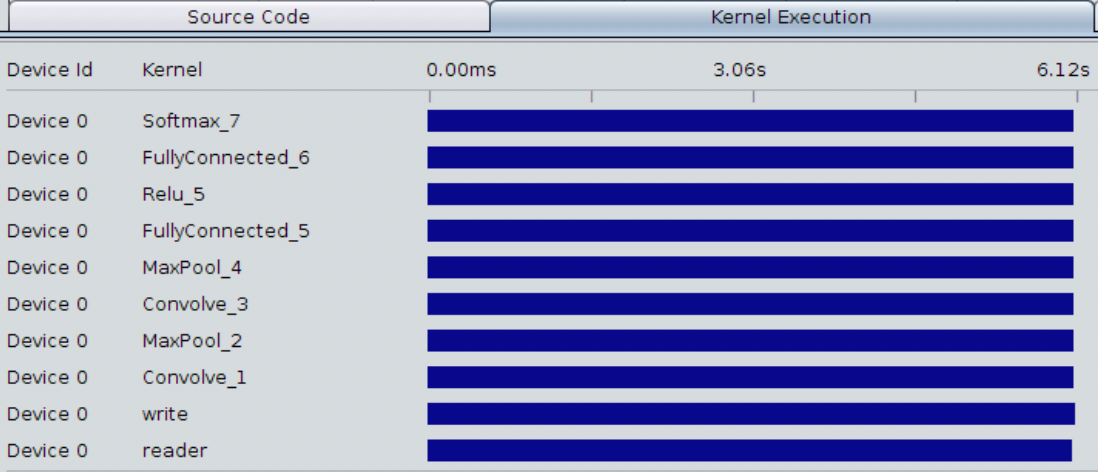
\includegraphics[width=0.85\textwidth]{Figures/pipebatch}
\decoRule
\caption[pipebatch]{ Execution time for inference of a batch of images (pipelined)}
\label{fig:pipebatch}
\end{figure}

\begin{figure}[h!]
\centering
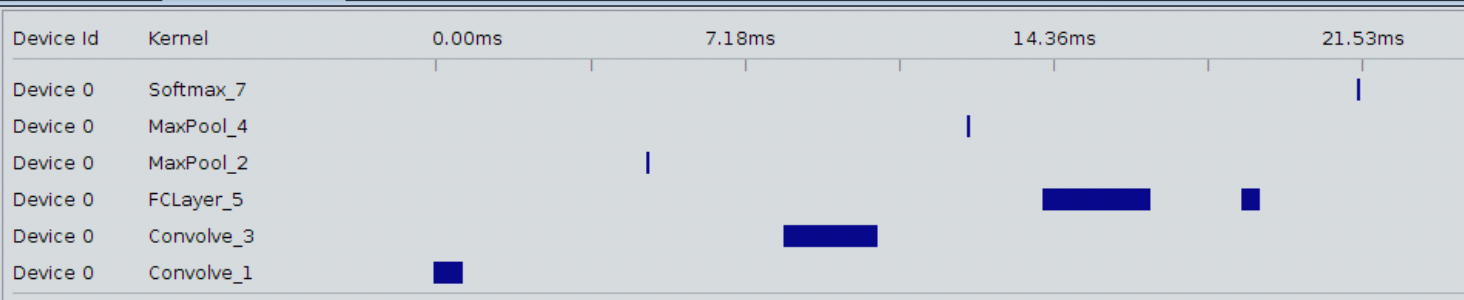
\includegraphics[width=0.85\textwidth]{Figures/nonpipesingle}
\decoRule
\caption[nonpipesingle]{ Execution time for inference of a single image (non-pipelined)}
\label{fig:nonpipesingle}
\end{figure}

\begin{figure}[h!]
\centering
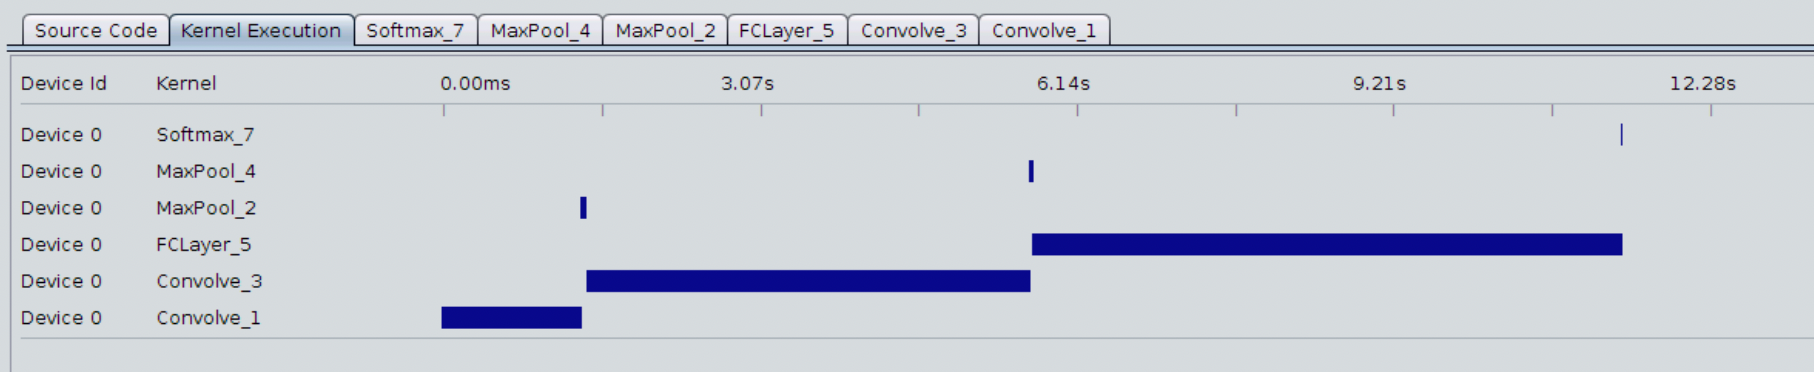
\includegraphics[width=0.85\textwidth]{Figures/nonpipebatch}
\decoRule
\caption[nonpipebatch]{ Execution time for inference of a batch of images (non-pipelined)}
\label{fig:nonpipebatch}
\end{figure}

%----------------------------------------------------------------------------------------

\newpage
\section{Training LeNet}

\subsection{Reconfiguration Time}

We implemented full minibatch backpropagation for the LeNet model. The problem we faced is that the fully optimized kernel implementations for the forward and backward propagation do not fit in a single binary. The estimated area usage was always within the Arria 10's available resources and even less than 80\% logic utilization. However, the compiler would run out of memory or crash with random error messages during compilation after tens of hours of running. For that we chose to simplify the design and break it up into a binary for forward propagation and a binary for backpropagation. The FPGA would reconfigure when switching between the two modes and in this section we evaluate the feasibility of this appraoch.

\begin{figure}[h!]
\centering
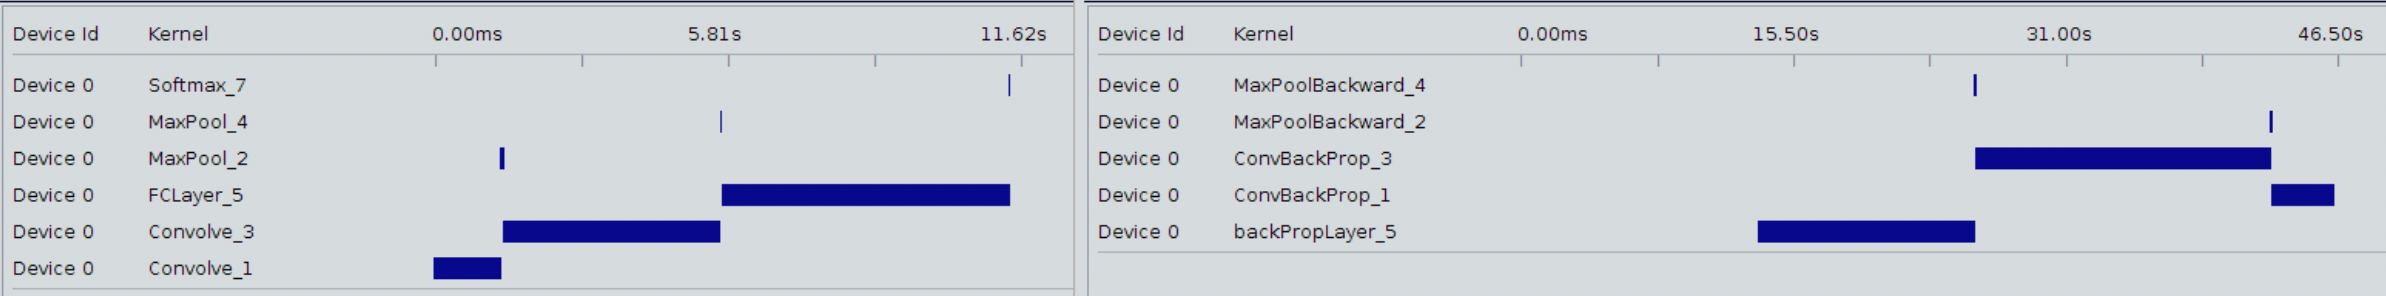
\includegraphics[width=1.0\textwidth]{Figures/fullprop}
\decoRule
\caption[fullprop]{ Dynamic Profiling results for minibatch on LeNet. }
\label{fig:fullprop}
\end{figure}

\begin{table}[]
\centering
\begin{tabular}{|c|c|c|c|}
\hline
\textbf{Batch Size} & \textbf{\begin{tabular}[c]{@{}c@{}}Total Epoch \\ Time\end{tabular}} & \textbf{\begin{tabular}[c]{@{}c@{}}Reconfiguration Time \\ (x2) in seconds\end{tabular}} & \textbf{\begin{tabular}[c]{@{}c@{}}$ \frac{Reconfiguration Time}{Total Epoch Time} $\end{tabular}} \\ \hline
1                   & 4.3                                                                  & 4.2                                                                                      & 97.6 \%                                                                                     \\ \hline
2048                & 49.1                                                                 & 4.6                                                                                      & 9.3\%                                                                                       \\ \hline
\end{tabular}
\caption{Reconfiguration Time Overhead}
\label{tab:reconfigure}
\end{table}


By looking at Fig. \ref{fig:fullprop} and after re-running the experiment time for multiple times, we realize that reconfiguration time is long and takes between 2 and 2.5 seconds in total. For a small batch size or in the case of a single image, reconfiguration time introduces a large overhead. When working with large batches, the effect is minimized ( as shown in Table \ref{tab:reconfigure} ). One iteration in the table consists of kernel reconfiguration ( twice ), forward propagation, and backward propagation with weight updates for the full batch.

In the case of a batch size of 2048, the overhead of reconfiguration is still large (9.7\%), however this is more feasible to perform as opposed to a single image. Nevertheless, with larger batch sizes, we risk reaching a local minimum when optimizing the loss function as discussed before in \ref{graddesc}.

\subsubsection{Challenges}

The implementation of LeNet required a lot of modifications until we started to see a decrease in the loss function. One of the challenges was the vanishing gradient problem \cite{hochreiter1998vanishing}. We solved this by replacing the ReLU function with the leaky ReLU which improved the training procedure. The Leaky ReLU function is given by \ref{lrelu}.
 \begin{equation}
  f(x) = \left\{
  \begin{array}{lr}
    x & : \textrm{if } x \ge 0 \\
    0.01x & : otherwise
  \end{array}
\right.
\label{lrelu}
 \end{equation}
 In back-propagating the error in the fully connected layers, we experimented with gradient clipping techniques which also improved the stability in the weight updates. 

We ran the batch size of 2048 on the FPGA, however it took as long as  ~2 hours per epoch and we did not get an improvement in accuracy. This may be due either to the batch size being too large, or because of some error introduced into the minibatch backpropagation implementation for convolutional layers. 

As for simply running Stochastic Gradient Descent,  it is unfeasible to run on the FPGA due to the overhead of reconfiguration which dominates runtime. Therefore, to test SGD, we used the Intel Emulator and noticed a decrease in the loss function but we did not run it until convergence as the emulator crashes when too many threads are launched and destroyed. 

\subsection{Simple Classifier}

\begin{table}[]
\centering
\begin{tabular}{|l|l|l|}
\hline
\textbf{Layer}           & \textbf{No. of Neurons} & \textbf{Trainable Parameters} \\ \hline
\textit{Input}           & 784 ( 28*28 )           & 0                             \\ \hline
\textit{Fully Connected} & 512                     & 401,920                       \\ \hline
\textit{Fully Connected} & 512                     & 262,656                       \\ \hline
\textit{Fully Connected} & 10                      & 5130                          \\ \hline
\textit{Softmax}         & 10                      & 0                             \\ \hline
\end{tabular}
\caption{Number of Trainable Parameters per Layer in the Simple Classifier.}
\label{tab:simplemod}
\end{table}

For additional verification, we compiled a simple neural network composed of only fully connected layers. The number of neurons per layer is shown in Table \ref{tab:simplemod}. We trained the model until convergence and unlike the LeNet model, both the full forward and backward propagation fit on the Arria 10 FPGA. 
It achieved reasonable runtime, $\approx$5.3 minutes per epoch and took 20 epochs to converge. We randomly sampled 5000 images of the MNIST Dataset for training and 500 images for testing. Eventually, the model achieved 67\% test error. 

In the simple model there is a \textbf{lot} of room to tune hyperparameters. Moreover, in this experiment, we did not aim to come up with the highest accuracy or fastest runtime.  The goal was to prove the correctness and the usability of the framework in a case where both forward and backward propagation fit on a single board configuration. Hopefully with a more advanced board, with a better fabric we can achieve better performance for more complex models.

%----------------------------------------------------------------------------------------
 
%% Chapter 4

\chapter{Intel OpenCL SDK Primer} % Main chapter title

\label{Chapter5} %

%----------------------------------------------------------------------------------------

\section{Development Workflow}

The standard workflow recommended by the Intel OpenCL programming guide\cite{progguide} is to compile a kernel for emulation in order to verify correctness. The software emulation that Intel offers mimics the real deployment of a kernel in production and requires writing a host program to control the kernel program ( as in a typical OpenCL deployment ). This overhead of the host program includes writing code for creating and launching a kernel, allocating and managing buffer space, and a lot of overhead platform detection code which makes the overall development process slower. For that we follow a different approach to developing OpenCL kernels in order to improve functional testing for correctness during the initial stages of kernel compilation.

 As OpenCL is a C-based language, kernels can be fully compiled using GCC asides from the OpenCL  API specific calls. This may appear counter-intuitive as OpenCL has a different programming model, but for FPGAs we are usually writing kernels as a single Work item as opposed to NDRange kernels \cite{opencl}. Knowing this, we are not explicitly using the programming model’s thread parallel execution paradigm. This means that kernels can be compiled and tested as ordinary C-functions as a single work item that follows a sequential C programming style. This also makes it easier to use gdb for debugging any issues with the kernel before emulation and creating a host program. 
 
 To fully enable this feature we have abstracted the OpenCL specifics using macros as a first step. In the small example in \ref{code:abstraction}, the \emph{kernel} keyword informs the OpenCL compiler that this function is a kernel and not an ordinary function. We don't need this specifier when compiling for C using GCC so we specialize it only for Intel's OpenCL compiler. This is one way to allow multiple compilers to compile the same file for different objectives. Another way is to use templating engines for our files so we leave this as future work.
 
\lstinputlisting[style=CStyle, caption={simple example of abstracting API specifics}]{code/kernel.c} \label{code:abstraction} 
  
We have automated this abstraction process and extended it to several other features like OpenCL channel communication. For that, we overrode Intel's channel API \cite{intel2016sdk} functions like \emph{read\textunderscore channel\textunderscore intel()} and \emph{write\textunderscore channel\textunderscore intel()} and direct those to reads and writes from a thread-safe implementation of \emph{blocking queues}. The overriden functionality is again only introduced when the kernel is compiled with GCC and not the Intel compiler. When testing with multiple kernels, each kernel is launched in a separate thread and we can successfully emulate a multi-threaded environment and can debug errors in communication between the kernels such as queue starvation or overflow. 
Template files would be a another option for abstracting those specifics, so we leave this as future work for now. This development workflow serves as a first step to writing generic C-functions with cross-platform support.

\section{Single Work-item vs ND-Range Kernel}

OpenCL’s view of shared memory fits more closely to GPUs than FPGAs, the need for portability of code for different architectures is still an ultimate goal that would enable efficient acceleration across different hardware devices. This is mainly why we see FPGA manufacturers like Altera and Xilinx improving the SDKs for supporting the development of FPGA kernels using OpenCL. Usually by using OpenCL’s programming model \cite{opencl}, parallelism can be achieved by exploiting the ND-range kernel feature to parallelize a lot of work. Parallelization is done when the work is split up into multiple work groups consisting of work items. This division can be represented along one, two, or even three dimensions. This parallelization is useful and makes coding easier as the inputs and intermediate feature maps in the case of a convolutional neural networks are multidimensional and can easily be split. This splitting allows the GPU to execute these kernels simultaneously on separate processors. 

In terms of supporting this, an FPGA has a fixed architecture and cannot invoke copies of the same kernel dynamically through a host program. Moreover, the specification by Intel recommends the use of single work-items when there are memory dependencies between the different work items. Synchronization in an NDrange programming model will thus result in pipeline flushes thus decreasing the pipeline efficiency. For that full efficiency can be better achieved by using the single-work item model. For example shift registers can only be inferred only in the single-work item as we need to have a main loop that accepts input and performs the shift operation at every iteration. For that, we use only single work-item kernels in our work as this allows us to perform multiple optimizations that are only possible at compile time and not host-program runtime. 

In case, thread level parallelism is required, and there are no interdependencies, this can be done by wrapping the function in a loop and unrolling over the computation which provides a more efficient implementation in hardware. 

\section{Inferring Shift-Registers} \label{shiftinf}

We discussed before how one of the convolution implementations \ref{fig:sliding buffer} relies on a shift-register for storing a sliding window of the input feature map. The trick to make that work is to create a loop that does the shift operation and ( move all items by one position ) and then explicitly specify the \emph{unroll} pragma so that the compiler an perform this optimization. An example is shown in listing \ref{code:shift}.

\newpage

\lstinputlisting[style=CStyle, caption={Shift Register Inference}]{code/shiftreg.c} \label{code:shift} 

\section{Reconfiguring the FPGA}

Some tasks may requires reprogramming an FPGA during runtime. The Intel FPGA specifies very little about reprogramming a kernel during host runtime. Since reprogramming takes a considerably large time ($\approx100ms-700ms $), it doesn’t make sense to trigger this feature often. We have used this feature in training a neural network with large batch sizes to minimize the delay introduced by reconfiguration. In the training experiment we compiled the forward and backward propagation kernels into two separate binaries as they were too large to be synthesized together in the same design. It is suitable only when batching with large sizes such as 2048 so that reprogramming time is minimal with respect to actual compute time. 

Our advice for this to work is that one must make sure to finish running kernels by running $ clFinish(queue) $ on all of the task queues and cleanup resources in a separate $ cleanup()$ procedure when switching between configurations. The cleanup procedure should clear all buffers used by the kernels, then the kernels themselves. The program binary then has to be recreated with the second kernel through a call to $createProgramFromBinary()$ . Under the hoods, this function creates a handle to the device and reprograms it given the binary string of the new kernel we wish to use. Also it is not guaranteed that when re-allocating buffers in global memory that they will contain the same old values, therefore one must make sure to transfer everything in global memory back and forth between the device and the host when reconfiguring separate kernels.

\section{Loops}

The general advice for loops is that the less loops the better. When working with multidimentional grids it is natural to use multiple nested loops, however this decreases the efficiency of the static code optimizer. We introduce a workaround for collapsing nested loops into a single loop. This optimization was also discussed by \cite{2018combined}. For example a nested loop \ref{code:loopa} can be collapsed to onw loop as in \ref{code:loopb}.

\begin{minipage}{0.5\textwidth}
  
\lstinputlisting[style=CStyle, caption={nested loops, src\cite{2018combined}}]{code/loopa.c} \label{code:loopa}   
  
\end{minipage}% This must go next to `\end{minipage}`
\vspace{0pt}
\hspace{5pt}
\begin{minipage}{0.5\textwidth}
 
\lstinputlisting[style=CStyle, caption={collapsed loops, src\cite{2018combined}}]{code/loopb.c} \label{code:loopb} 
 
\end{minipage}

This allows the optimizer to better resolve the loop exit conditions and enable it to resolve the condition in one clock cycle. Also the nested structures require additional hardware to preserve state in between iterations. It is also better practice to limit variables to the scope of variables to only where they are used and not in higher level loops and collapsing loops can be a measure against this.


\section{Loop-Carried Memory Dependencies} \label{loopdep}

When using OpenCl, it is easy forget that we are not developing a CPU application, so we tend discard unnecessary data structures and we do not consider memory dependencies in between instructions. When programming an FPGA however, it is important to relieve memory dependencies within iterations in order to get an optimal pipelined structure scheduled with an iteration interval $ ii=1 $ . Memory dependencies introduce stalls into the dataflow must wait until the result of a previous iteration is ready before proceeding to the next instruction. 

For that we can use local memory to relieve dependencies and hold intermediate results, after that reductions can be performed on this local storage and the overall pipeline would become more efficient on the expense of a higher resource usage. A simple example in Intel's Best Practices Guide \cite{intelsdk} shows how one can use a register to hold intermediate results and relieve the loop-carried dependencies. We extend Intel's example when the requirement is to have a mix of pipelining and unrolling of an inner loop. Unrolling in an inner loop increases the critical path for the loop carried dependencies. 

To overcome this problem, our solution consists of combining two optimizations. The first step is to transfer the dependency from global memory to a local register. The second step is to compile with the \emph{-fp-relaxed} compiler option so that the reduction on the local register is relaxed and performed in a tree-style adder without dependencies \ref{code:nondep}. 

\newpage

\lstinputlisting[style=CStyle, caption={Loop-carried dependencies}]{code/dep.c} \label{code:dep}   
  
\lstinputlisting[style=CStyle, caption={Dependencies are transferred to a local register}]{code/nondep.c} \label{code:nondep} 

In some cases, we do not wish to use the \emph{-fp-relaxed} because we care about the numerical stability in other places in the code. In that case the memory dependency can be transferred to a local array of registers, and a reduction can be transferred on that array \ref{code:nondeptwo}. This is effectively implementing the \emph{-fp-relaxed} option on part of the code. We use this solution in our convolution operation as we also perform additional processing on the intermediate array of registers.

\newpage

\lstinputlisting[style=CStyle, caption={Dependency transferred to a local array}]{code/nondeptwo.c} \label{code:nondeptwo} 


\section{Using Multiple Queues}

In order to execute multiple kernels concurrently, one must instantiate multiple command queues and enqueue the concurrent tasks separately within the same program. This is especially important for concurrent kernels that communicate through channels \cite{intel2016sdk}. Multiple queues should be considered in the emulation stage as well, since the emulator processes tasks sequentially, unless there are multiple queues involved, then it launches multiple threads to consume from the different queues at the same time.


%---------------------------------------------------------------------------------------- 

%----------------------------------------------------------------------------------------
%	THESIS CONTENT - APPENDICES
%----------------------------------------------------------------------------------------

\appendix % Cue to tell LaTeX that the following "chapters" are Appendices

% Include the appendices of the thesis as separate files from the Appendices folder
% Uncomment the lines as you write the Appendices

% Appendix A

\chapter{Frequently Asked Questions} % Main appendix title

\label{AppendixA} % For referencing this appendix elsewhere, use \ref{AppendixA}

\section{How do I change the colors of links?}

The color of links can be changed to your liking using:

{\small\verb!\hypersetup{urlcolor=red}!}, or

{\small\verb!\hypersetup{citecolor=green}!}, or

{\small\verb!\hypersetup{allcolor=blue}!}.

\noindent If you want to completely hide the links, you can use:

{\small\verb!\hypersetup{allcolors=.}!}, or even better: 

{\small\verb!\hypersetup{hidelinks}!}.

\noindent If you want to have obvious links in the PDF but not the printed text, use:

{\small\verb!\hypersetup{colorlinks=false}!}.

%\include{Appendices/AppendixB}
%\include{Appendices/AppendixC}

%----------------------------------------------------------------------------------------
%	BIBLIOGRAPHY
%----------------------------------------------------------------------------------------


\printbibliography[heading=bibintoc]

%----------------------------------------------------------------------------------------

\end{document}  
